\part{Mechanics}
The first semester is all about the study of mechanics, the study of how physical bodies interact with their environments. An understanding of mechanics is crucial since it serves as the foundation from which the rest of physics is built.  

\section{Building Blocks}
\subsection{Mathematics Excursion I: Calculus}
Before we dive head-first into mechanics, we have to establish our ground rules. Over the course of this handout, we will be using calculus extensively/pretty much everywhere. Some of the prouder physicists would say calculus was invented to deal with mechanics in the first place! In this vein, it's important that we at least have some understanding of what calculus is and how to use it. 

It's okay if this section doesn't make complete sense if you haven't taken a calculus course -- this section is mostly intended to highlight a few important concepts, and as a reference as you proceed through the rest of the handout. You will definitely want to consult other texts to learn and practice calculus more extensively -- TJHSST uses \textit{Early Transcendentals} by Anton, Bivens, and Davis, of which copies can certainly be found online, although we do not condone or encourage the use of piracy to obtain educational materials. 

There are two main parts of single-variable calculus -- differential calculus (dealing with derivatives) and integral calculus (dealing with integrals). We'll look at these two as well as some of the more common applications of calculus to solve problems.
\subsubsection{Derivatives}
Derivatives describe how a function is changing over time. We may as well call it the "slope" of the function - ie. how much a function's output changes with respect to the input. For a function $f$ that is a line, the derivative of the function really is just the slope of the line, because remember that the slope for a line $y = mx+b$ is:
\[
	f'(x) = \dv{f}{x} = \dv{}{x}f(x) = m = \frac{\Delta y}{\Delta x} 
\]	
which is exactly the ratio of the change in the output to the change in the input.\\
The first three expressions are basically equivalent ways to write "the derivative of the function $f$ with respect to $x$." Whatever you want to use is up to you to denote the derivative, but I tend to use different notations depending on the situation. 
\begin{center}
	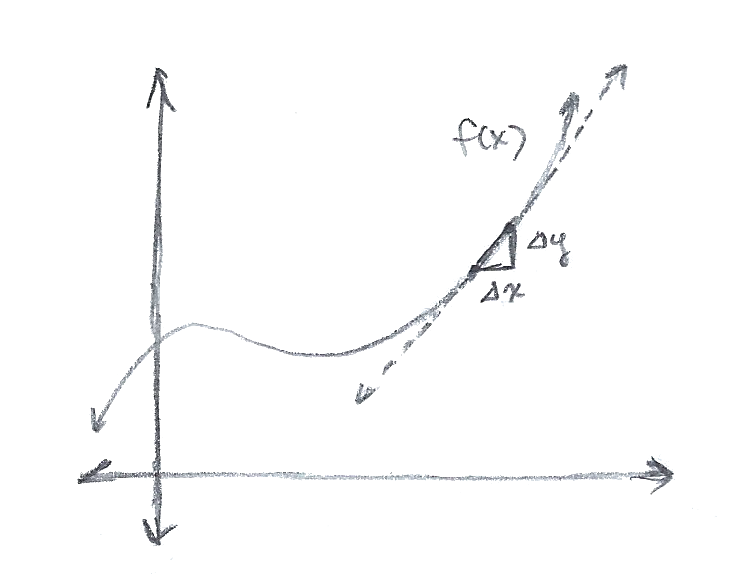
\includegraphics[scale=0.3]{images/math/calc/derivative.png}
\end{center}
What about for non-linear functions? We can still look at how a function's $y$-value changes due to small changes in $x$. If the change in $x$ is small enough, the region of the function around any $x$-value looks kind of like a line anyways. We can find an approximate value for the derivative of a function by looking at the value of the function on the interval $[x, x+h]$, where $h$ is some small real number: 
\[
	\dv{f}{x} \approx \frac{f(x+h) - f(x)}{x+h - x} = \frac{f(x+h) - f(x)}{h}
\]
To get the derivative of $f$, we let the value of $h$ go to zero, to see how the function changes instantaneously. Of course, we can't let $h$ equal zero, because that would be dividing by zero - but we can look at how this expression behaves for values of $h$ close to zero. This is the idea behind taking a limit, which in general allow you to look at what functions do as they approach certain values of $x$ (which you should have learned in TJ Math 5). 
\[
	\dv{f}{x} = \lim_{h\to 0} \frac{f(x+h) - f(x)}{h}
\]
This is the definition of the derivative of $f$ with respect to $x$. With this limit definition, we can start to compute the derivative for more complex functions. Let's look at the derivative of $f(x) = x^2$:
\[
	\dv{f}{x} = \lim_{h\to 0} \frac{f(x+h) - f(x)}{h} =  \lim_{h\to 0} \frac{(x+h)^2 - x^2}{h} =  \lim_{h\to 0} \frac{x^2 + 2xh + h^2 - x^2}{h} = \lim_{h\to 0} \frac{2xh + h^2}{h} = \lim_{h\to 0} 2x+h = 2x
\]
In general, it can be proven that if $f(x) = x^n$, for any real value of $n$: 
\[
	\dv{f}{x} = nx^{n-1}
\]	
This is called the power rule for derivatives. If $n$ is an integer, you can use the binomial theorem - but I'll leave that proof for you to discover. \\
Derivatives also satisfy the following properties, provable from the definition of the derivative:
The derivative of a sum or a multiple of two functions is the same as the sum or a multiple of the derivative of the functions. (This property is called linearity.) 
\[
	\dv{}{x}(f(x) + g(x)) = f'(x) + g'(x) \quad \dv{}{x}(cf(x)) = cf'(x) 
\]
For constant functions $f(x) = c$, we can see that 
\[
	\dv{f}{x} = \dv{}{x} (c) = 0
\]
For the product of functions, we can invoke the product rule, which states that:
\[
	\dv{}{x}(f(x) \cdot g(x)) = f'(x) g(x) + f(x) g'(x)
\]
Closely related is the quotient rule, which is applied for the quotient of two functions:
\[
	\dv{}{x}\left(\frac{f(x)}{g(x)}\right) = \frac{f'(x) g(x) - f(x) g'(x)}{g(x)^2}
\]
Most important of all is the chain rule for the composition of two functions $f(x)$ and $g(x)$:
\[
	\dv{}{x}f(g(x)) = \dv{f}{g} \cdot \dv{g}{x}
\]
What we mean by this notation is that wherever $g(x)$ is substituted in place of $x$ in $f(x)$, we take the derivative of $f(x)$ as if $g(x)$ were the variable, and then multiply by the derivative of $g(x)$ with respect to $x$. It would probably be more clear if I showed you a basic example - Let's look at the derivative of $f(x) = (3x+2)^2$. Let's evaluate this by expanding and taking the derivative of each term:
\[
	\dv{f}{x} = \dv{}{x} (9x^2 + 12x + 4) = 18x + 12
\]
Let's do this using the chain rule, assuming we're looking at the composition of the functions $x^2$ and $3x+2$:
\[
	\dv{f}{x} = 2(3x+2)^{1} \cdot 3 = 18x + 12
\]
The proof of the chain rule is the most complicated, and you can find proofs of all of these facts online. Using the limit definition, we can derive the derivatives of trigonometric, exponential, and logarithmic functions. I've listed them all here in a table:
\begin{center}
	\begin{tabular}{cc|cc|cc}
		\multicolumn{2}{c}{Trigonometric}&\multicolumn{2}{c}{Exponential}&\multicolumn{2}{c}{Inverse Trig}\\ \hline \hline \noalign{\smallskip}
		Function & Derivative & Function & Derivative & Function & Derivative \\ \hline \noalign{\smallskip}
		$\sin x$ & $\cos x$ & $e^x$ & $e^x$ & $\arcsin x$ & $\frac{1}{\sqrt{1-x^2}}$ \\ \hline \noalign{\smallskip}
		$\cos x$ & $-\sin x$ & $\ln x$ & $\frac{1}{x}$ & $\arccos x$ & $-\frac{1}{\sqrt{1-x^2}}$\\ \hline \noalign{\smallskip}
		$\tan x$ & $\sec^2 x$ & $a^x$ & $a^x \ln a$ & $\arctan x$ & $\frac{1}{1+x^2}$\\ \hline \noalign{\smallskip}
		$\cot x$ & $-\csc^2 x$ & $\log_a x$ & $\frac{1}{x \ln a}$ & $\arccot x$ & $-\frac{1}{1+x^2}$ \\ \hline \noalign{\smallskip}
		$\sec x$ & $\sec x \tan x$ & $c^f$ & $c^f \ln c\cdot f'$ & $\arcsec x$ & $\frac{1}{|x|\sqrt{x^2-1}}$ \\ \hline \noalign{\smallskip}
		$\csc x$ & $-\csc x \cot x$ & $f^{g}$ & $f^g \left(f'\frac{g}{f} + g' \ln f \right)$ & $\arccsc x$ & $-\frac{1}{|x|\sqrt{x^2-1}}$ \\ \hline \noalign{\smallskip}
	\end{tabular}
\end{center}
(The function $f(x) = e^x$ is defined so that its derivative is itself. The derivatives of other exponential functions are derived from the chain rule.) Using these principles, we can take the derivative of any elementary function and find out what it's rate of change using these rules.\\
We can also keep taking the derivative of the function as many times as we want, as long as the function is differentiable (meaning that the function is continuous and the limit involved in the derivative exists). We've only looked at the first derivatives of functions so far, but we can always find the second derivatives, third derivatives, etc. of functions. Notation-wise, we use $\dnv{y}{x}{n}$ for the $n$th derivative of a function, or $f^{n}(x)$ where $n$ is either expressed in Roman numerals if $n < 4$ or just written out regularly (which is in my opinion super arbitrary). Usually, however, we rarely go beyond the second derivative in physics. 

\subsubsection{Indefinite Integrals}
Given a function $f(x)$, let's try to find the function $F(x)$ that has $f(x)$ as its derivative. $F(x)$ is called the antiderivative of $f(x)$. We write $F(x)$ as the following:
\[
	F(x) = \int f(x) \, dx 
\]
The $dx$ at the end means that the antiderivative is being found with respect to the variable $x$. The big $\int$ symbol is called an integral, and finding the antiderivative is called taking the indefinite integral (or the integral, for short) - which is what I'll call it from now on, to avoid typing so much. \\
In general, it's much more difficult to integrate functions, and most of the time, the integral of a random composition of functions cannot be expressed as a combination of elementary functions. Let's just look at a simple example to start - the integral of $f(x) = x^2$. We can use a little bit of trial and error to do this. Notice that because of the power rule for derivatives, the exponents in polynomial functions decrease by 1. Therefore, we know that the antiderivative $F(x)$ has to be of the form $F(x) = kx^3$. By definition, 
\[
	\dv{}{x} F(x) = \dv{}{x} \int f(x) \, dx = f(x) 
\]
We know that $\dv{}{x} F(x) = 3 kx^2 = f(x)$. Therefore, $k = \frac{1}{3}$, so at the end of it all, we have:
\[
	F(x) = \int x^2 \, dx  = \frac{1}{3}x^3 + C
\]
Why add the $+C$? Because the derivative of a function eliminates the constant (the derivative of a constant is zero), any constant could have been added to the original function $F(x)$ to produce a derivative of $f(x)$. We can add any constant we want, but if we want to be as general as possible, we use a $+C$ represents any real number.\\
We don't have as many properties that hold in general for the evaluations of all integrals, but at least the properties of linearity still hold. That is, for any two functions, the integral of the sum or constant multiple of these functions is the sum or the constant multiple of the integral of the function:
\[
	\int f(x) + g(x) \, dx = \int f(x) \, dx + \int g(x) \, dx \quad \int cf(x) \, dx = c \int f(x) \, dx
\]
Here's a table of the most common integrals so you can get started: 
\begin{center}
	\begin{tabular}{c c}
		\multicolumn{2}{c}{Most Common Integrals}\\ \hline \noalign{\smallskip}
		Function & Antiderivative \\ \hline \hline \noalign{\smallskip}
		$\int x^n \, dx$ & $\frac{1}{n+1}x^{n+1}$ + C\\ \noalign{\smallskip} \hline \noalign{\smallskip}
		$\int e^x \, dx$ & $e^x + C$ \\ \noalign{\smallskip} \hline \noalign{\smallskip}
		$\int a^x \, dx$ & $\frac{1}{\ln a} a^x + C$ \\ \noalign{\smallskip} \hline \noalign{\smallskip}
		$\int \sin x \, dx$ & $-\cos x + C$ \\ \noalign{\smallskip} \hline \noalign{\smallskip}
		$\int \cos x \, dx$ & $\sin x + C$ \\ \noalign{\smallskip} \hline \noalign{\smallskip}
		$\int \sec^2 x \, dx$ & $\tan x + C$ \\ \noalign{\smallskip} \hline \noalign{\smallskip}
		%$\int \sec x \tan x \, dx$ & $\sec x + C$ \\ \noalign{\smallskip} \hline \noalign{\smallskip}
		$\int \tan x \, dx$ & $\ln |\sec x| + C$ \\ \noalign{\smallskip} \hline \noalign{\smallskip}
		$\int \frac{1}{x}\, dx$ & $\ln |x| + C$ \\ \noalign{\smallskip} \hline \noalign{\smallskip}
		$\int \frac{1}{\sqrt{1-x^2}} \, dx$ & $\arcsin x + C$ \\ \noalign{\smallskip} \hline \noalign{\smallskip}
		$\int \frac{1}{1+x^2}\, dx$ & $\arctan x + C$ \\ \noalign{\smallskip} \hline \noalign{\smallskip}
	\end{tabular}
\end{center}	
We do have some other tricks that we can use to evaluate more complex integrals. The most powerful is called the $u$-substitution, and it changes the variables inside the integral. Essentially, it's like the reverse of the chain rule, and works for integration. Let's just look at an example -  the integral $\int xe^{x^2} \, dx$. At first, this may seem really hard to do - after all, we don't know a function that has this as a derivative from the table, but what we can do is substitute $u = x^2$. When we do this, however, we also have to substitute in a new variable of integration (also called a differential) $du = 2x \, dx$. This is computed by taking the derivative of the substituted expression - note that $\dv{u}{x} = 2x$, so we just "multiply through" by $dx$. We substitute in $\frac{1}{2} u = x\, dx$ so we get:
\[
	\int xe^{x^2} \, dx = \int \frac{1}{2} e^u \, du = \frac{1}{2} e^u + C
\]
We can't leave our answer in terms of $u$, so we substitute back in to get: 
\[
	\int xe^{x^2} \, dx = \frac{1}{2}e^{x^2} + C
\]
Selecting the proper $u$-substitution for an integral can make the difference between making your job difficult and making your job easy. It takes a lot of practice to find the right $u$-substitution to simplify the integral to one of the most common integrals. \\
Another effective tool for evaluating integrals that involve products of functions. For functions $u$ and $v$ with differentials $du$ and $dv$, we have that:
\[
	\int u\, dv = uv - \int v \, du
\]
This is called the technique of integration by parts. For products of functions, even if the integral $\int u\, dv$ is hard to evaluate, we can transform it such that the new integral $\int v \, du$ is easier to evaluate. Let's look at the integral $\int x \sin x \, dx$. This is really hard to integrate on its own, but we can consider the products of the functions $u(x) = x$ and $v = -\cos x$. The differentials of these functions are $du = dx$ and $dv = \sin x \, dx$. If we plug this into the integration by parts formula, we have: 
\[
	\int x \sin x \, dx = -x \cos x - \int (- \cos x) \, dx = -x \cos x + \int \cos x \, dx
\]
We can evaluate the right side of the equation a bit more easily:
\[
	- x \cos x + \int \cos x \, dx = - x \cos x + \sin x + C
\]
Therefore, we have: 
\[
	\int x \sin x \, dx = -x \cos x + \sin x + C
\]
Our selection of $u$ and $v$ is a skill that can be improved with experience doing integrals. Usually, $u$ is a function that needs to be easily differentiated, and $dv$ needs to be easily integrated in order for the new integral to be easily evaluated. \\
A few other techniques that we will may look at throughout the course of the handout are using partial fractions to evaluate integrals and trigonometric substitution. We will address them as needed.

\subsubsection{Definite Integrals and the Fundamental Theorem of Calculus}
We can represent the accumulation of a quantity using a definite integral, and it has a close relation to the area that a function encloses. 
\begin{center}
	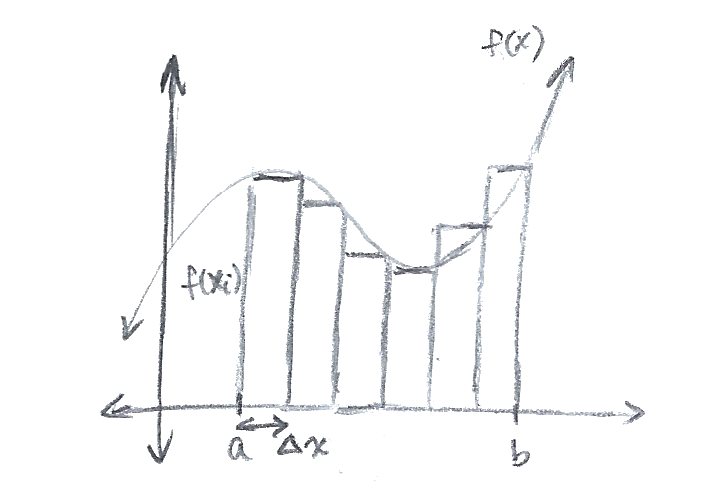
\includegraphics[scale=0.3]{images/math/calc/defintegral.png}
\end{center}
The area $A$ between the curve of $f(x)$ and $x-axis$ on the interval from $x = a$ to $x=b$ can be represented by a sum of many rectangles. If we subdivide the interval $[a,b]$ into $N$ equal intervals of length $\Delta x$, we can construct a rectangle in each interval that has width $\Delta x$ and height $f(x_i)$, where $x_i$ is the right-most $x$-coordinate of each interval. The area under the curve can be approximated by these rectangles. We can write this as:
\[
	A \approx \sum_{x_i \in [a,b]} f(x_i) \, \Delta x
\]
If we let the number of rectangles go to infinity and the width of each rectangle go to zero, we can approach the actual area of the curve. Therefore, we can write the area as a limit:
\[
	A = \lim_{N\to \infty , \Delta x \to 0} \sum_{x_i \in [a,b]} f(x_i) \, \Delta x = \int_a^b f(x) \, dx
\]
This is the definition of the definite integral, also called the Riemann integral. \\
We can also relate this to the indefinite integral. If $f(x)$ is the function that represents the rate of change of a function $F(x)$ with respect to $x$, every small rectangle in the area underneath the curve represents a small change in the value of $F(x)$. This is because that area represents the value of rate of change of $f(x)$ multiplied by the small change in $x$ ($dx$), which is the net change in $F(x)$, $\Delta F(x)$:
\[
	\Delta F(x) = f(x) \, dx
\]
If all of these small changes are summed up, the result is the net change in the function $F(x)$ on the interval $[a, b]$. Therefore, we can write the definite integral of a function $f(x)$ on the interval $[a, b]$ as the following:
\[
	\int_a^b f(x) \, dx = F(x)\Big|_a^b = F(b) - F(a) 
\] 
This is called the Fundamental Theorem of Calculus. We can now evaluate definite integrals by finding the antiderivative using an indefinite integral. This is incredibly useful for evaluating definite integrals, which we will do a lot during physics. 

\subsubsection{Differential Equations}
One of the applications for calculus is to create a model of a situation when the only information given is based on how things are changing at any particular point. Differential equations help us do this - they relate the derivatives of a function to the function itself. What if we want to do find a solution to a differential equation - that is, find an explicit expression for the function without involving its, given a few data points? This is extremely difficult in the general case, but in physics we will usually look at a few easier cases. \\
For the most part, we will be looking at first-order differential equations, where the only terms with derivatives involve the first derivative of the function. The most basic case is when the first derivative of a function only involves the independent variable $x$ (or $t$, $\theta$, etc.) and doesn't involve the function in the equation. For an example of this, let's look at the following function of $y$, assuming that we know that $y(0) = 1$:
\[
	\dv{y}{x} = e^{x} - 4x
\]
To solve it, we can just integrate with respect to $x$ from $0$ to some arbitrary real $r$: 
\[
	\int_0^r \dv{y}{x} \, dx = \int_0^r \, dy = \int_0^r e^{x} - 4x \, dx
\]
\[
	y(x)\Big|_0^r = (e^x - 2x^2)\Big|_0^r
\]
\[
	y(r) - y(0) = e^r - 2r^2 - 1
\]
\[
	y(r) = e^r - 2r^2 - 1 + y(0)
\]
Now, we see that the specific solution of the function that we're looking for depends on a data point. Since we know that $y(0) = 1$, we can simply plug in this value to get:
\[
	y(x) = e^x - 2x^2
\]
Since there's nothing special about our choice of $r$, it's simply standing in as a dummy variable - so I can replace it with $x$ or really anything I want. If I had changed the value of our initial data point, we could have had any arbitrary constant added onto the end of this, and it still would satisfy the original differential equation. In general, however, adding a constant to the end of any solution to a differential equation won't necessarily always allow it to satisfy the original equation. Let's look at another example: 
\[
	\dv{y}{x} = xy 
\]
In this case, we have the original function involved, so just integrating won't work. However, we can "separate" the variables by moving everything with a $y$ to one side and everything with an $x$ in it to another: 
\[
	\frac{1}{y} \, dy = x \, dx
\]
Now we can integrate with respect to each differential:
\[
	\ln |y| = \frac{1}{2}x^2 + C
\]
We can now solve for $y$:
\[
	y = e^{\frac{1}{2}x^2 + C} = Ce^{\frac{1}{2}x^2}
\]
Notice that because of the exponentiation, you can only manipulate the constant as a scale factor and not as an added constant. If you try substituting this back into the original equation, you can see that it works in general, whereas if you try adding a constant to the function instead it won't work. \\
In the text, I solve differential equations by moving all the terms to one side and integrating, which is essentially the same as separation of variables and results in the same solutions. Separation of variables is generally better for finding general solutions, but I use a shortcut for plugging in the data point to create the specific solution to match the situation. 

\subsubsection{Taylor Series Expansions}
The final tool that we use for solving problems are Taylor series. I claim that if a function is differentiable to an arbitrarily large degree at a point, I can approximate the behavior of the function as a polynomial at that point. (For simplicity, we'll assume that this point is at $x=0$.)\\
To create a polynomial that matches the behavior of the function at a point, all of the derivatives of the function at the point should match that of the polynomial. Let's be more specific - say the function is $f(x)$, and we know the values of $f(0), f'(0), f''(0),$ etc. We can try to build a function $p(x)$ that matches the $n$th-derivative at $x=0$. \\
If we just want to match $f(x)$ at $x=0$, we could just have $p(x) = f(0)$. This isn't a very good approximation of the function everywhere, though - it only matches the function at this point. Let's try again. \\
If we also want to make $p'(x)$ match $f'(x)$ at $x =0$, we could use a line - consider $p(x) = f(0) + f'(0) x$. Notice that this function has derivative $p(x) = f'(0)$, so it works. \\
Let's keep going to the second derivative. We want to add a term, but also make sure that the added term doesn't mess up what we had before. Because after taking two derivatives only polynomial terms of degree 2 will be constant, the added term should look like $kx^2$ for some $k$. If we take two derivatives of this term, the constant term that's left should look like $2k$ (because of the power rule). In order for us to have the right second derivative at $x = 0$, the coefficient $k = \frac{f''(0)}{2}$. So far, then, $p(x) = f(0) + f'(0)x + \frac{f''(0)}{2}x^2$ will match $f(x)$ for the first two derivatives and the value of $f(0)$. \\
We can continue on like this. The polynomial $p(x) = f(0) + f'(0)x + \frac{f''(0)}{2} x^2 + \frac{f'''(0)}{6} x^3$ will match $f(x)$ at the first three derivatives at $x=0$ (show this yourself) and we can keep adding on to infinity, basically. In general, we can make an infinite polynomial as follows that will be exactly $f(x)$:
\[
	f(x) = \sum_{i=0}^{\infty} \frac{f^{i}(0)}{i!}x^i
\]
This infinite polynomial is called the Taylor series of $f(x)$. A lot of the time, we will approximate functions using Taylor series if their inputs are close to zero. In these scenarios, we will basically just appproximate the first non-zero term to be the value of the function close to zero. Let's look at the function $\sin x$ (a function that we will approximate a lot) and compute the derivatives of $\sin x$ at $x=0$:
\[
	\sin (0) = 0
\]
\[
	\dv{}{x} \sin x = \cos x \rightarrow \dv{}{x} \sin x \Big|_{x=0} = \cos (0) = 1
\]
\[
	\ddv{}{x} \sin x = -\sin x \rightarrow \ddv{}{x} \sin x \Big|_{x=0} = -\sin (0) = 0
\]
\[
	\dnv{}{x}{3} \sin x = -\cos x \rightarrow \dnv{}{x}{3} \sin x \Big|_{x=0} = -\cos (0) = -1
\]
\[
	\dnv{}{x}{4} \sin x =  \sin x \rightarrow \dnv{}{x}{4} \sin x \Big|_{x=0} =  \sin (0) = 0
\]
Since the derivatives of $\sin x$ basically cycle through every four derivatives, we know that the Taylor series of $\sin x$ is:
\[
	\sin x = 0 + 1 \cdot x + \frac{0}{2} x^2 + \frac{-1}{6}x^3 + \frac{0}{24}x^4 + \ldots = \sum_{i = 0}^{\infty} \frac{(-1)^i}{(2i+1)!}x^{2i+1}
\]
The first non-zero term you see here is $x$, so we commonly approximate $\sin x = x$ for $x$ close to zero. (And now hopefully you understand math memes a little better.) \\
Taylor series are pretty important - although we don't use them in the text, some of the problems do require their use in order to solve them. 
\pagebreak

\subsection{Kinematics}
We begin our study of mechanics by trying to quantify the behavior of moving objects. Specifically, we will look at how objects' position, velocity, and acceleration are related, and how these can be used to solve problems involving motion, especially in certain special cases. 
\subsubsection{General Motion}
Moving forward, we will describe an object's position using a vector with respect to some point, denoted $\vec{r}$. For simplicity, we will use a point as our moving particle, but principles here really apply to any object. \\
\begin{center}
	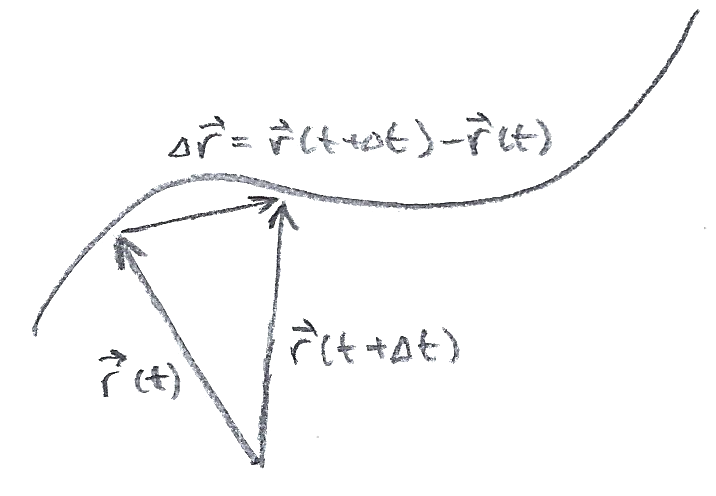
\includegraphics[width=0.5\textwidth]{images/mechintro/general_motion.png}\\
\end{center}
Knowing the position of the object is great, but we would definitely like to know more about a particle than just its position. For example, how do we know how fast is the particle going? Intuitively, we can find the average velocity of a particle over an interval by taking the distance traveled over the time interval. Consider the particle at two different times, with positions $\vec{r}(t)$ and $\vec{r}(t + \Delta t)$. Define the displacement of the particle as $\Delta\vec{r} = \vec{r}(t + \Delta t) - \vec{r}(t)$. Using the displacement vector, we can find the average velocity (a vector): 
\[
	\vec{v}_{av} = \frac{\Delta \vec{r}}{\Delta t} = \frac{\vec{r}(t + \Delta t) - \vec{r}(t)}{\Delta t}
\]
Average velocity is nice, but we would like to know the velocity instantaneously. Notice as we shrink the time interval $\Delta t$, our average velocity becomes more and more like the instantaneous velocity $\vec{v}$. In the limit as $\Delta t \rightarrow 0$, we have:
\[
	\vec{v} = \lim_{\Delta t \rightarrow 0} \frac{\vec{r}(t + \Delta t) - \vec{r}(t)}{\Delta t}
\]
This looks rather like the derivative of the position vector function $\vec{r}(t)$ with respect to time! However, we don't really know how to take the derivative of a vector, but we \textit{should} know how to take the derivative of an arbitrary function. We can actually do this by splitting the position vector $\vec{r}(t)$ into $xy$-components, where $\vec{r}(t) = x(t) \hat{x} + y(t) \hat{y}$ and $\vec{r}(t+\Delta t) = x(t+\Delta t) \hat{x} + y(t+\Delta t) \hat{y}$:
\begin{align*}
	\vec{v}(t) &= \lim_{\Delta t \rightarrow 0} \frac{x(t+\Delta t) \hat{x} + y(t+\Delta t) \hat{y} -x(t) \hat{x} -y(t) \hat{y}}{\Delta t}\\
	&= \lim_{\Delta t \rightarrow 0} \frac{x(t+\Delta t)-x(t)}{\Delta t} \hat{x} + \lim_{\Delta t \rightarrow 0}\frac{y(t+\Delta t)-y(t)}{\Delta t} \hat{y}\\
	&= \dv{x}{t}\hat{x} + \dv{y}{t} \hat{y} = v_x\hat x + v_y \hat y
\end{align*}
Note that $v_x = \dv{x}{t}$ is the $x$-component of the velocity, and $v_y = \dv{y}{t}$ is the $y$-component of the velocity. We can do this process again to attain the instantaneous acceleration vector $\vec a$, noting that the average acceleration is the change in the velocity vector over a time $\Delta t$ and allowing $\Delta t$ to go to $0$:
\[
	\vec a = \dv{v_x}{t}\hat x + \dv{v_y}{t} \hat y = \ddv{x}{t} \hat x + \ddv{y}{t} \hat y
\]
We normally don't deal with any derivatives of position (with respect to time) of order higher than two. Also, usually we will deal with constant-acceleration motion and constant-velocity (zero acceleration) motion, with some special exceptions. More general cases will be dealt with later when we discuss energy. \\
Let's deal with the constant-velocity case right now. Because of the Fundamental Theorem of Calculus, we can note the following: 
\[
	x(t) - x_0 = \int_0^t v_x \, dt = v_xt \rightarrow x(t) = v_xt + x_0
\]
where the last step follows from noting that the velocity is a constant, and therefore so are each component of the velocity vector. Using similar relations for the $y$-coordinate, we have: 
\[
	\vec r(t) = \vec v t + \vec r_0
\]
We don't need any other information about constant-velocity problems - since the velocity is constant, all higher order derivatives must be zero.\\
Now we look at the constant-acceleration case, starting with the acceleration vector $\vec a$. We can use the Fundamental Theorem of Calculus again, as we did with the constant-velocity case: 
\[
	v_x(t) - v_{0_{x}} = \int_0^t a_x \, dt = a_xt \rightarrow v_x(t) = a_xt + v_{0_{x}}
\]
Repeating this again, we can find the $x$-coordinate of position:
\[
	x(t) - x_0 = \int_0^t v_x \, dt = \int_0^t v_{0_{x}} + a_xt \, dt = v_{x0}t + \frac{1}{2}at^2  \rightarrow x(t) = x_0 + v_{0_{x}}t + \frac{1}{2}at^2
\]
Using similar processes for the $y$-coordinate, we have
\[
	\vec{r}(t) = \vec r_0 + \vec v_0 t + \frac{1}{2} \vec{a} t^2 
\]
\[
	\vec v(t) = \vec a t + \vec v_0
\]
where $\vec r_0$ is the initial position vector, $\vec v_0$ is the initial velocity vector, and $\vec a$ is the acceleration vector. \\
These equations work fine unless we don't have access to time data. However, we can derive a constant-acceleration equation that does not involve time, using one dimension for simplicity. We can square our general equation for velocity: 
\begin{align*}
	v &= at + v_0 \\
	v^2 &= a^2t^2 + v_0^2 + 2atv_0 \\
	v^2 - v_0^2 &= 2a\left(\frac{1}{2}at^2 + v_0t \right)
\end{align*}
This expression in the parentheses is familiar - note the displacement can be written as:
\[
	\Delta x = x(t) - x_0 = \frac{1}{2}at^2 + v_0t
\]
Now we have a kinematic equation that does not deal with time: 
\[
	v^2 - v_0^2 = 2a\Delta x
\]
Note that these equations are the same in higher dimensions (for example, in 3D space) and are derivable with the same procedures and steps. 

\subsubsection{Circular Motion}
A special type of motion that we will study is circular motion. In order to derive the equations for this motion, we use polar coordinates. We can parameterize the points in the plane with the angle it makes with the positive $x$-axis and the distance from the origin. Let $\theta(t)$ be this angle as a function of time, and we can express the position of a point in the plane as $\vec r = r \cos (\theta (t)) \, \hat x + r \sin (\theta (t)) \, \hat y$, where $r$ is the constant radius of the circle the particle travels upon. In addition to $\hat x$ and $\hat y$, constant unit vectors, we define changing unit vectors $\hat r$ and $\hat \theta$, where $\hat r$ is radially outward and $\hat \theta$ is the unit vector perpendicular to it, defined as follows: \\
\[
	\hat r = \cos (\theta (t)) \, \hat x + \sin (\theta (t)) \, \hat y 
\]
\[
	\hat \theta = -\sin (\theta (t)) \, \hat x + \cos (\theta (t)) \, \hat y
\]
\begin{center}
	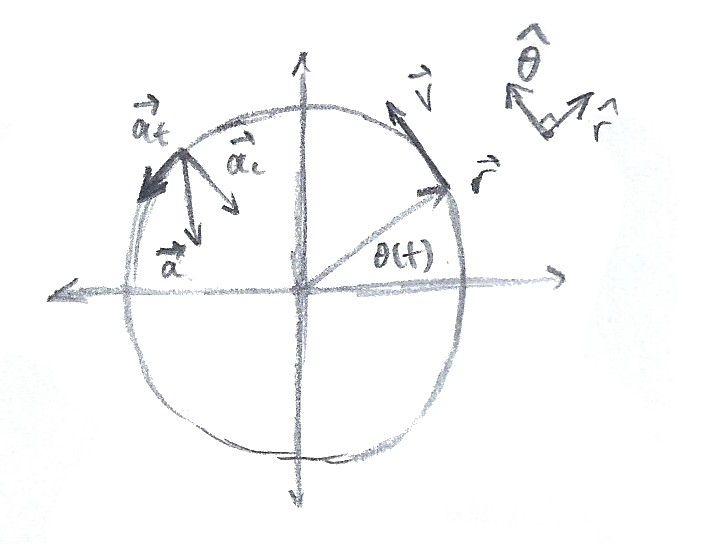
\includegraphics[width=0.5\textwidth]{images/mechintro/circular_motion.png}\\
\end{center}
We can take the derivative of the position vector in order to find the velocity of the object, using the method in the previous section: 
\[
	\vec v = \dv{\vec r}{t} = - r \sin (\theta (t)) \, \dv{\theta}{t} \, \hat x + r \cos (\theta (t)) \, \dv{\theta}{t} \, \hat y
\]
Notice by the chain rule an extra $\omega = \dv{\theta}{t}$ appears in each term; this term is called the angular velocity. We can rewrite $\vec v$ as follows: 
\[
	\vec v = \omega r (-\sin (\theta (t)) \, \hat x + \cos (\theta (t)) \, \hat y) 
\]
The acceleration of the object is a bit messy, but we can take derivatives again, substituting $\alpha = \dv{\omega}{t}$: 
\begin{align*}
	\vec a = \dv{\vec v}{t} &= -r \left(\dv{\omega}{t}\sin (\theta (t)) + \omega^2 \cos (\theta (t)) \right) \hat x + r \left(\dv{\omega}{t} \cos (\theta (t)) - \omega^2 \sin (\theta (t)) \right) \hat y \\
	&= \alpha r (-\sin (\theta (t)) \, \hat x + \cos (\theta (t)) \, \hat y) - \omega^2 r (\cos (\theta (t)) \, \hat x + \sin (\theta (t)) \, \hat y) 
\end{align*}
This is all pretty messy, but we can clean up these expressions by using $\hat r$ and $\hat \theta$: 
\begin{align*}
	\vec r &= r \hat r \\
	\vec v &= \omega r \hat \theta \\
	\vec a &= \alpha r \hat \theta - \omega^2 r \hat r
\end{align*}
Observe that since these unit vectors have magnitude $1$, so the velocity $v = \omega r$, with direction tangent to the circle. We should notice for cases with non-constant acceleration, we have a centripetal component ($-\omega^2 r \hat r$, pointing radially inward) and a tangential component ($\alpha r \hat \theta$, tangent to the circle).
A special case we study is when $\omega$ is a constant, implying that $\alpha = 0$. This is called uniform circular motion, and we see for this case the only acceleration is centripetal: 
\[
	\vec a = - \omega^2 r \hat r = - \frac{v^2}{r} \hat r 
\]
Overall, we have, for uniform circular motion (for the magnitudes of the velocity and angular velocity):
\begin{align*}
	v &= \omega r \\
	a &= \omega^2 r = \frac{v^2}{r}
\end{align*}

\subsubsection{Simple Harmonic Motion (SHM)}
Consider projecting circular motion into one dimension - namely, only considering the $x$-direction. This one-dimensional motion can basically be modeled by the function $x(t) = A \cos(\omega t + \phi)$, where $A$ is the amplitude, $\omega$ is the frequency/angular velocity, and $\phi$ is the phase shift. This is simple harmonic motion, which essentially uses a sine/cosine function as a model for motion. \\
Using our knowledge of derivatives, the velocity and acceleration functions: 
\begin{align*}
	v(t) &= -\omega A \sin(\omega t + \phi) \\
	a(t) &= -\omega^2 A \cos(\omega t + \phi) 
\end{align*}
We'll do something somewhat unorthodox - we'll substitute $x(t)$ for the cosine function in the acceleration function, giving: 
\[
	a(t) = \ddv{x}{t} = -\omega^2 x(t)
\]
In general, if given an acceleration function proportional to position, where $a(t) = -kx(t)$, we know the particle exhibits simple harmonic motion (sine/cosine wave) where $\omega = \sqrt{k}$ and the period $T = \frac{2\pi}{\omega} = \frac{2\pi}{\sqrt{k}}$. \\
Mathematically, if a second derivative of a function $\ddv{f}{t} = -kf$, the function $f$ can be modeled as a sine or cosine function. 

\subsubsection{Projectile Motion and Relative Motion}
We can apply general 2-D motion principles to projectiles. Let a particle be launched at an angle $\theta$ at an initial velocity $v_0$. Note that this particle is constantly accelerating downward with magnitude $g = 9.81 \, m/s^2$. To make things simpler, we will automatically project into the $x$- and $y$- directions, with the implication that we are in fact dealing with vectors. Also, further assumptions that we make is that the Earth's gravitational acceleration is uniform at all heights - which clearly isn't true in outer space - but otherwise we have non-constant acceleration which we haven't learned to deal with yet. We also neglect air resistance, which changes the acceleration of the particle. \\
The initial velocity in the $x$-direction is $v_0 \cos \theta$, and the initial velocity in the $y$-direction is $v_0 \sin \theta$. Plugging into our derived time-dependent kinematic equations, and letting the initial position be the origin: 
\[
	x(t) = v_0t\cos\theta  \quad v_x(t) = v_0\cos\theta
\]
\[
	y(t) = v_0t\sin\theta  - \frac{1}{2}gt^2 \quad v_y(t) = v_0 \sin \theta - gt
\]
We can analyze some critical points - we can calculate how far the particle will travel before it hits the ground, namely when $y = 0$. When this is the case, we have: 
\[
	v_0t\sin\theta  - \frac{1}{2}gt^2 = 0 \rightarrow v_0\sin\theta - \frac{1}{2}gt = 0
\]
This equation has a zero when $t=0$, and solving the remaining linear equation yields $t = \frac{2v_0\sin\theta}{g}$. When this is plugged into $x(t)$, we have $\frac{2v_0^2\sin\theta \cos\theta}{g} = \frac{v_0^2\sin 2\theta}{g}$.\\
Similarly, we can consider when the particle reaches its maximal height. Clearly, by symmetry we have that the distance that the particle had traveled to that point is $\frac{v_0^2\sin \theta \cos\theta}{g}$. However, we can find the maximal height by calculating the time when the $y$-component of the velocity is $0$, where the particle stops going upward and begins to fall back to earth. This occurs when:
\[
	v_0\sin\theta - gt = 0 \rightarrow t = \frac{v_0\sin\theta}{g}
\]
Note that the time when this occurs is exactly half of the time it takes for the particle to hit the ground. When this occurs, the height can be calculated by plugging into $y(t)$, where $y(t) =\frac{v_0^2\sin^2\theta}{2g}$. \\
Of course, this is all well and good, but we do need to be able to consider when things hit each other, especially with projectiles (which is a very common problem). \\
\begin{center}
	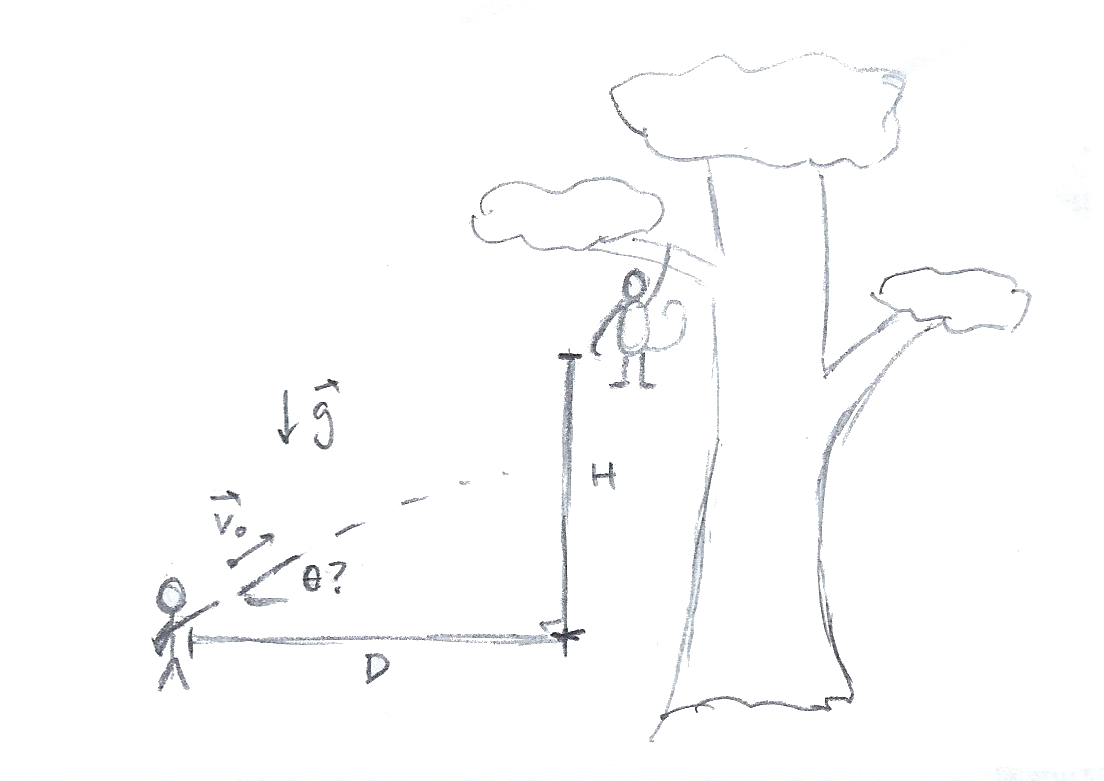
\includegraphics[width=0.5\textwidth]{images/mechintro/projectile_motion.png}\\
\end{center}
We can use kinematics to solve problems - one of the first applications was used for hunting, because animal cruelty organizations didn't exist when physics was invented. For example, suppose a hunter stands a distance $D$ away from the base of a tree, in which a monkey is sitting at the top, hanging from a branch. The monkey is hanging at a height $H$, and the hunter can shoot a bullet at the monkey with velocity $v_0$. We're trying to find at what angle $\theta$ should the hunter fire to hit the monkey. We're also assuming the monkey is effectively a point, and at the instant the hunter fires, the monkey lets go of the branch and begins to fall freely with downward acceleration with magnitude $g$.\\
Consider the position vector of the monkey relative to the bullet, $\vec r_{MB}$. To deal with this, we employ the following, where $O$ is some arbitrary origin we've been using the entire time:
\[
	\vec r_{BO} + \vec r_{MB} = \vec r_{MO} \rightarrow \vec r_{MB} = \vec r_{MO} - \vec r_{BO} 
\]
To compute the relative position vector, then, we really only need to 
compute the position vectors of the monkey and the bullet and subtract them. We know they collide when their relative position vector is the zero vector $\vec 0$.  We know how both of these particles work - effectively, they are both projectiles, which we have just established. For simplicity, let the position of the hunter be the origin. Then, we have: 
\[
	\vec r_{MO} = D\, \hat x + \left(H - \frac{1}{2}gt^2 \right)\, \hat y \quad \vec r_{BO} = v_0t\cos\theta \, \hat x + \left(v_0t\sin\theta - \frac{1}{2} gt^2 \right) \, \hat y
\]
Then their relative position is: 
\[
	\vec r_{MB} = (D - v_0t\cos\theta) \, \hat x + (H - v_0t\sin\theta) \, \hat y
\]
When this is the zero vector, we have that both components are zero, giving:
\[
	\cos \theta = \frac{D}{v_0t} \quad \sin \theta = \frac{H}{v_0t} \rightarrow \tan \theta = \frac{H}{D}
\]
This angle is the exact angle at which the hunter should shoot the monkey hanging from the tree, given our assumptions. Therefore, the hunter should aim directly at the monkey, as long as the bullet is traveling fast enough to reach the tree before the monkey hits the ground. 

\subsubsection{Summary and Problems}
Position, velocity, and acceleration of objects can be represented by a vector with respect to a point. Velocity is the derivative with respect to time of position, and acceleration is the derivative with respect to time of velocity (and the second derivative with respect to time of position). Position and velocity can be attained through velocity or acceleration functions, respectively, through integration. \\
We deal with a few special cases, being (uniform) circular motion, simple harmonic motion, and projectile motion. These are situations that we should be proficient in before moving forward to more complex motion and systems. \\

\noindent \textbf{Problems:}\\
1. (3 $\bigstar$) At $1/2$ of its maximum height, the speed of a projectile is $3/4$ of its initial speed. If the particle was initially launched at an angle $\theta$, where $\theta = \arctan(x)$, show that $x = \sqrt{7}$.\\
2. (2 $\bigstar$) A boy whirls a stone in a horizontal circle of radius $r$ and at height $h$ above ground level. The string breaks, and the stone flies horizontally and strikes the ground after traveling a horizontal distance of $d$. Show the magnitude of the centripetal acceleration of the stone while in circular motion is $d^2g/2hr$. \\
3. (2 $\bigstar$) Two particles oscillate in simple harmonic motion along a common straight-line segment of length $A$. Each particle has a period of 3.80 s, but they differ in phase by $\pi/8$ rad. a) Show the maximum acceleration and velocities of the particles are 2.734$A$ and 1.653$A$, respectively. b) Show the particles are 0.167$A$ apart $0.50$ s after the lagging particle leaves one end of the segment.\\
4. (1 $\bigstar$) A tank fires a rocket at a velocity $v_r$ at an angle $\theta$ above the horizontal. Immediately afterward, the tank begins moving forward at a constant speed $v_t$. Show that the angle of stupidity $\theta$ of the tank - that is, the angle at which the rocket will fall down to strike the tank while on the ground - as $\arccos(v_t/v_r)$. \\
5. (3 $\bigstar$, $\spadesuit$) A small rock sinking through water experiences an exponentially decreasing acceleration given by $a_y(t) = ge^{-bt}$, where $b$ is a positive constant that depends on the shape/size of the rock and the properties of the water. If the initial position and velocity of the rock are both zero, find the a) velocity function to be $v_y(t) = \frac{g}{b} (1-e^{-bt})$. b) the position function to be $y(t) = \frac{g}{b}t - \frac{g}{b^2}(1-e^{-bt})$.\\
6. (2 $\bigstar$) Prove that if two particles are launched at the same speed $v_0$ but at angles above the horizontal that exceed/fall short of 45 degrees by the same amount, they will still travel the same distance (on level ground).\\
7. (3 $\bigstar$) If two balls are thrown with the same initial speed $v_0$ but at different angles $\alpha$ and $\beta$ above and below the horizontal, respectively, and from a cliff a height $h$ above the ground, show that their velocities right before they hit the ground are the same and is equal to $v = \sqrt{v_0^2+2gh}$.\\

\pagebreak

\subsection{Dynamics and Newton's Laws}
Once we have the tools to deal with motion to some level, we now begin to deal with how interactions between objects influence motion - specifically, with the use of forces. Forces have units of kg $\cdot$ m/s$^2$, also denoted as N, called the newton in honor of Isaac Newton. One newton (1 N) of force is the amount needed to accelerate a 1 kg mass by 1 m/s$^2$. 
\subsubsection{The Laws of Motion}
When Newton developed his theory of dynamics for the first time, he established the quantity of linear momentum, $P$, representing the motion of a mass particle. He defined it as:
\[
	\vec P = m \vec v
\]
Forces, he said, were the flow of linear momentum in between objects in contact. Objects in contact with each other are interacting, delivering this momentum to each other. These forces can be represented as vectors, delivering this momentum from place to place. \\
With this in mind, this means force is the derivative of the linear momentum with respect of time, and we obtain the iconic second of Newton's three laws of motion, regarding all forces acting on a particle:
\[
	\sum_i \vec F_i = \dv{\vec P}{t} = m \dv{\vec v}{t} = m \vec a
\]
However, we have to be careful about how we use this law. In physics, since we can't analyze the whole universe in one go, we only look at subsections of the universe called reference frames, from which we can analyze the physical situation. If a reference frame has any added external forces to a system, they will change the motion of an object within - this is Newton's first law. An object's velocity, whether at rest or positive, will be changed by the addition of an external force. This means that in order to maintain consistency, we cannot analyze objects that lie in reference frames that are accelerating and expect them to be consistent with the results obtained from a stationary measurement since some external force is causing them to accelerate. Therefore, we only analyze objects in inertial reference frames, that is, a reference frame that does not change the inertia or momentum of the system. \\
To illustrate this, let's imagine Dr. Dell in his brand-new Tesla, on the highway. He accelerates, and as he does so, he notices sheep, standing in a pasture, as he passes by. Relative to him, Dr. Dell sees the sheep accelerating backward, and concludes there must be some force in that direction that makes them move this way. However, if I stand next to these sheep in the field, clearly I see them at rest. The laws of physics do not apply arbitrarily, in order to maintain a consistent image of the universe.\\
Forces primarily come from objects that come into contact with one another. When two objects interact, they exert forces on each other, and they do so with equal magnitude in opposite directions. This is Newton's third law, the establishment of the existence of these forces called action-reaction pairs. For example, if a book is sitting on a table, the book is exerting a downward force on the table, but the table is also exerting an upward force on the book. However, the force of gravity on the book is not an action-reaction pair with the upward force from the table! Even though the two forces are opposite in direction and have the same magnitude, gravity is a result of an interaction with the Earth, which means it cannot be paired with the force from the table.\\
To briefly sumamrize Newton's Laws of Motion: 
\begin{mdframed}[frametitle=Newton's Laws of Motion]
	1. In a system with no internal forces, an object's velocity can only be changed by some external force.\\
	2. Force is the flow of linear momentum between objects, and thus forces on an object have the same direction as the net acceleration of an object.\\
	3. Particles that interact with each other have forces exerted on each other that are opposite in direction but equal in magnitude. 
\end{mdframed}
Not only are there contact forces, however, there are also action-at-a-distance forces that we have not yet considered. These also follow Newton's Second Law but seem to come from nowhere (a problem that we still don't really know the answer to today!). We include them when drawing free-body diagrams, where we list all the possible forces that act on an object, such as gravity, the electromagnetic force (discussed in length later), and the strong and weak nuclear forces (not discussed). In mechanics, we mostly concern ourselves with gravity, a largely macroscopic force. In problems that are assumed to be on Earth, gravity does exert an external force on the system, so strictly speaking, the Earth is not an inertial frame! However, we will still apply Newton's laws in these systems, and just automatically consider gravity acting on the system where applicable. 
\subsubsection{The Sandbox}
In many problems, certain common objects occur in systems that have well-known properties that students must know in AP Physics. 
\begin{mdframed}[frametitle=The Gravitational Force]
	Earth exerts an action-at-a-distance force on all objects on its surface. This force has magnitude $mg$, where $m$ is the object's mass, $g$ is the acceleration due to gravity ($9.81 m/s^2$) and is directed straight down.
\end{mdframed}
\begin{mdframed}[frametitle=The String and The Tensile Force]
	For ideal strings that are effectively massless, and stretched taut, the tension in the string acts as a contact force on the object in the direction of the string outward from the object. The magnitude of this force is the same for all objects attached to the string. 
\end{mdframed}
\begin{mdframed}[frametitle=The Normal Force]
	The contact force from a surface exerted on an objects when touching each other perpendicular to the surface. It is part of an action-reaction pair with force from the object on the surface, but not with the force of gravity on the object. 
\end{mdframed}
\begin{mdframed}[frametitle=The Frictional Force]
	A contact force that opposes the motion of objects. Friction comes in two types - static friction and kinetic friction. \\
	Static friction is for objects at rest and has a magnitude $f_s \leq \mu_sN$, where $N$ is the magnitude of the normal force and $\mu_s$ is the coefficient of static friction (between $0$ and $1$). This force opposes an applied force on an object until the magnitude of this force exceeds the maximum magnitude of the static frictional force, at which point the object will begin to move.\\
	Kinetic friction opposes the motion of a moving object and has magnitude $f_k = \mu_kN$, where $\mu_k$ is the coefficient of kinetic friction (also between 0 and 1, usually smaller than $\mu_s$). This force points in the exact opposite direction of the velocity of the object to decelerate the object. 
\end{mdframed}
\begin{mdframed}[frametitle=The Elastic Force]
	The elastic force, usually exerted by a spring in problems, has magnitude $\vec F_{spring} = -k \Delta \vec x$, where $\Delta \vec x$ is the displacement of the object attached to the spring from equilibrium, and $k$ the spring constant. Note that this force opposes compression/stretching of the spring. Without any other forces on this system, objects attached to a spring move in simple harmonic motion. 
\end{mdframed}
\begin{mdframed}[frametitle=The Drag Force]
	The force of drag on an object is $F_d = \beta v^n$, where $\beta$ is the coefficient of drag, $v$ is the velocity, and $n$ is some arbitrary real ($n=2$ through air and many other fluids). This force opposes motion through the air, and we usually don't consider this force because it has a negligible impact on results on the scale of the lab. 
\end{mdframed}
\subsubsection{Atwood's Machine}
The most common example that requires the application of Newton's Laws is Atwood's machine, which is essentially a pulley with two masses hanging from both ends of a string wrapped around it. The string does not slip on the pulley and is effectively massless, and for now, the pulley is fixed and does not rotate with the string (this is a non-trivial constraint that we will talk about later). \\
\begin{mdframed}[frametitle=Atwood's Machine]
Consider Atwood's machine with masses $m_1$ and $m_2$, and $m_2 > m_1$. Find the acceleration of the blocks and the tension in the string in terms of $m_1, m_2, g$, where $g$ is the acceleration due to gravity.
\end{mdframed}
The first thing we need to do is figure out what forces are acting on both blocks. We're not considering air resistance, and no friction is acting between the pulley and the string, so we can ignore these contact forces. The most helpful tool we use in these problems is a free-body diagram, which illustrates the forces acting on each object. Here are the free body diagrams for both of the blocks: 
\begin{center}
	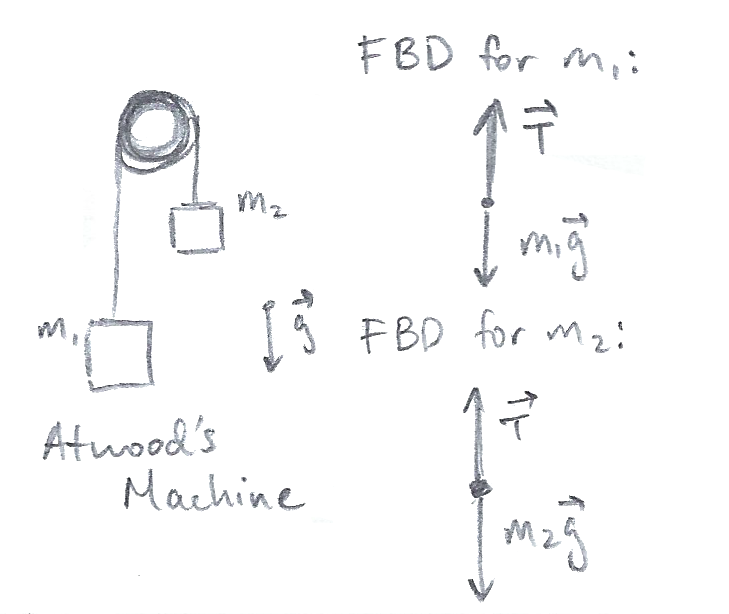
\includegraphics[width=0.5\textwidth]{images/mechintro/atwoods_machine.png}\\
\end{center}
Note that the forces only act in one direction, so we will establish a unit vector $\hat y$ upwards in order to project the components of the forces along this line. First, we do need to write Newton's Second Law for each block: 
\[
	\sum_i \vec F_i = m_1 \vec g + \vec T = m_1 \vec a
\]
\[
	\sum_i \vec F_i = m_2 \vec g + \vec T = -m_2 \vec a
\]
The only subtlety here is noting that kinematically, the blocks are attached to each other and thus have the same acceleration, except in opposite directions - when one goes up, the other must go down, and vice versa, resulting in a negative sign in front of one of the equations. \\
Now we can project along the $y$-direction:
\begin{align*}
-m_1g + T = m_1a \\
-m_2g + T = -m_2a
\end{align*}
This is a two-variable system of equations with two unknowns, so we can just solve for $T$ and $a$, which aren't particularly pretty, but are:
\[
	T = \frac{2m_1m_2}{m_1+m_2}g \quad a = \frac{m_2-m_1}{m_2+m_1}g
\]

\subsubsection{Summary and Problems}
Newton's laws of motion can be applied to situations to analyze how objects move, especially when external forces are applied to systems of objects. We also can start to figure out how objects interact with each other based on their contacts with one another. \\
There isn't much to do other than to practice the method we use to analyze dynamical situations, that being to draw correct free-body diagrams, using Newton's Second Law and projecting into components, and then solving for all unknowns using some kinematics to simplify the number of variables involved.  \\

\noindent \textbf{Problems}\\
1. (1 $\bigstar$) a) A block of mass $m$, experiencing a force of friction, slides at constant speed down a plane inclined at an angle $\theta$ with the horizontal. Show $\mu_k = \tan\theta$. b) The same block rests on a frictionless wedge inclined at an angle of $\theta$. If the wedge is accelerated with acceleration $\vec a$ so that the block remains stationary relative to the wedge, show that the magnitude of this acceleration is $a = g\tan \theta$. \\
2. (3 $\bigstar$) A stone of mass $m$ attached to a string is whirled in a horizontal circle of radius $r$. The string makes an angle of $\theta$ with the vertical, and the other end of the string is fixed directly above the center of the circle. Show the speed of the stone is $v = \sqrt{rg\tan\theta}$ and the tension in the string is $T = mg/\cos\theta $.\\
3. (2 $\bigstar$) A slide-loving pig slides down a side with angle $\theta$ in $n$ times the time it would take to slide down a frictionless slide with angle $\theta$. Show that the coefficient of kinetic friction between the pig and the first slide is $\frac{n^2-1}{n^2}\tan\theta$.\\
4. (3 $\bigstar$) A puck of mass $m$ slides in a circle of radius $r$ on a frictionless table while attached to a hanging cylinder of mass $M$ by a cord through a hole in the table. Show if that the cylinder is to remain at rest, the puck needs to be moving at a speed of $v = \sqrt{\frac{Mgr}{m}}$. \\
5. (3 $\bigstar$, $\spadesuit$) Revisit Atwood's machine, in which two containers are connected by a cord (of negligible mass) passing over a frictionless pulley (also of negligible mass). At time $t = 0$, container 1 has mass 1.30 kg and container 2 has mass 3.36 kg, but container 1 is losing mass (through a leak) at the constant rate of 0.256 kg/s. a) Show that the rate at which the acceleration magnitude of the containers changing at $t = 3.00 \, s$ is 1.11 m/s$^3$. b) Show the acceleration reaches its maximum value at $t = 5.08$ s.\\
6. (2 $\bigstar$) The floor of a railroad flatcar is loaded with loose crates having a coefficient of static friction $\mu_s$ with the floor. If the train is initially moving at a speed of $v$, show the minimum distance $\Delta x$ in which the train can be stopped at constant acceleration without causing the crates to slide over the floor is $\frac{v^2}{2g\mu_s}$.\\
7. (5 $\bigstar$) A car travels on a banked curve. The coefficient of static friction between the tires of the car and the roadway of the banked curve is $\frac{3}{4}$. The curve has radius $R$ and is banked at the incline angle so that the force of static friction is zero if the car travels with constant speed $S$. Show that the maximum speed that a car can traverse the banked curve is $SRg \sqrt{\frac{7}{4-3S^2}}$. 

\pagebreak

\section{Conserved Quantities}
Aside from basic tools such as Newton's Laws or kinematics, when certain events occur we can analyze them using the conservation of certain physical quantities. This involves the use of linear momentum (that which forces are carriers of), angular momentum, and energy.

\subsection{Linear Momentum}
We mentioned linear momentum a bit in our discussion about forces, defining the product of an object's mass and velocity to be this quantity, as follows: 
\[
	\vec P = m \vec v
\]
where $\vec P$ stands for linear momentum. This is a vector quantity and has the same direction as the velocity and units of kg $\cdot$ m/s = N $\cdot$ s. 
\subsubsection{Impulse-Momentum Theorem}
Impulse is something that often comes up with discussions of linear momentum, and it would seem at first like a completely separate quantity. The impulse delivered to an object $\vec J$, in terms of the net force $\vec F$ on it over a time interval $[t_1, t_2]$ is defined to be the following: 
\[
	\vec J = \int_{t_1}^{t_2} \vec F \, dt
\]
Recall we can write the force $\vec F = \dv{\vec P}{t} = m \vec a$, so this becomes:
\[
	\vec J = \int_{t_1}^{t_2} \dv{\vec P}{t} \, dt = \vec P(t_2) - \vec P(t_1) = \Delta \vec P
\]
So, impulse is nothing terribly special - it's equal to the change in linear momentum delivered to a particle. This is also true in general for systems of particles - the total impulse delivered to a system is equal to the change in the total linear momentum of the system. This is the Impulse-Momentum Theorem, relating impulse to linear momentum. \\
We can go one step further. Notice that the average force on an object $\vec F_{av}$ is
\[
	\vec F_{av} = \frac{\Delta \vec P}{\Delta t}
\]
so the impulse delivered to the system over a time $\Delta t$ is just 
\[
	\vec J = \vec F_{av} \Delta t
\]
\subsubsection{Center of Mass}
The center of mass is a tool we need to use in order to use momentum effectively. From up until this point we have been operating under the assumption that objects effectively behave like a point particle. This really isn't true - after all, something like a baton when thrown into the air spins, and the motion of the end of the baton does not follow a perfect parabolic path as kinematics would have us believe. However, we know for certain that one point in the baton system follows this parabolic trajectory, being the center of mass. \\
First, let's just define the center of mass of a system of particles. Say with respect to some reference point these particles have position vectors $\vec r_i$, where $i$ goes from $1$ to however many particles there are. If each particle also has a mass $m_i$, and the mass of all of the particles is $M$, then the position of the center of mass $\vec r_{cm}$ is: 
\[
	\vec r_{cm} = \frac{1}{M} \sum_i m_i\vec r_i
\]
Essentially, this is a weighted average of the positions of each particle with respect to the mass. Since the masses are all scalars, we can take derivatives to find the velocity and acceleration of the center of mass, showing that these can also be found by taking the mass-weighted average of all the velocities and accelerations, respectively, of the particles. 
\[
	\vec v_{cm} = \dv{\vec r_{cm}}{t} = \dv{}{t} \frac{1}{M} \sum_i m_i \vec r_i = \frac{1}{M} \sum_i m_i \dv{\vec r_i}{t} = \frac{1}{M} \sum_i m_i \vec v_i
\]
\[
	\vec a_{cm} = \dv{\vec v_{cm}}{t} = \dv{}{t} \frac{1}{M} \sum_i m_i \vec v_i = \frac{1}{M} \sum_i m_i \dv{\vec v_i}{t} = \frac{1}{M} \sum_i m_i \vec a_i
\]
So how to find the center of mass? For a discrete collection of particles, the calculations are fairly straightforward - one just projects into components, and uses the same mass-weighted average to find the $x$-, $y$-, etc. components of the center of mass. Putting it all together with appropriate unit vectors gives the correct position vector. \\
For continuous distributions of mass, we have to be a bit more clever. If we let the mass of each little particle/subsection in a larger object go to zero as we divide it up into smaller and smaller pieces, then we can compute the desired sum as an integral by summing together all the appropriate pieces. This gives us:
\[
	\vec r_{cm} = \frac{1}{M} \int \vec r \, dm
\]
where $\vec r$ is the position vector of each infinitesimally small mass portion $dm$. 
Usually, when computing the center of mass for continuous distributions we define a density function $\lambda$, which represents mass per unit length. (AP Physics doesn't require being able to compute the center of mass for two/three/higher dimensional objects.) As a basic example, a rod with uniform density and mass $M$ and length $L$ has its center of mass in the middle of the rod, by symmetry. As a more nontrivial example, consider a semicircle with radius $R$ and uniform density (mass per unit length) $\lambda$.
\begin{center}
	\begin{asy}
		import olympiad;
		pair O, P, X;
        size(8cm);
		O = (0,0);
		dot(O);
		draw(arc(O, 1, 0, 180));
		real dtheta = 8;
		real angle = 40;
		X = dir(angle);
		P = dir(angle+dtheta);
		draw(O--P, linetype("8 8"));
		draw(O--X, linetype("8 8"));
		real vertoffset = -0.1;
		draw((0, vertoffset)--(-1, vertoffset), linetype("8 8"), arrow=Arrows());
        draw(dir(180)--dir(0), linetype("4 4"));
        draw(arc(O, 0.8, angle, angle+dtheta), arrow=Arrows());
        dot(2*dir(90)/pi);
        
        label("$\theta$", 0.15*dir(angle/2), dir(angle/2));
        label("$ds$", dir(angle+dtheta/2), dir(angle+dtheta/2));
        label("$R$", (-0.5, 1.2*vertoffset), dir(270));
        label("$d\theta$", 0.7*dir(angle-dtheta), dir(angle-dtheta));
        label("COM", 2*dir(90)/pi, NW);
	\end{asy}
\end{center}
Because the semicircle is uniform, we know that $\lambda = \frac{M}{\pi R}$, but we're not going to plug it into our expressions until the end. Let the $x$-axis be the diameter of the semicircle, and the $y$-axis the line through the center perpendicular to it. From here, we're going to use polar coordinates. \\
The vector $\vec r$ for all points on the semicircle is $R \cos \theta \, \hat x + R \sin \theta \, \hat y$, as $\theta$ ranges from $0$ to $\pi$. Now, we have to express $dm$ in terms of $\theta$. Note since each small piece is a small arc of the semicircle, $dm = \lambda \, ds$, where $ds$ is a small arc. We know that $ds = R \, d\theta$, so at the end of the day we have $dm = \lambda R \, d\theta$. Now, we can integrate and evaluate: 
\begin{align*}
	\vec r_{cm} &= \frac{1}{M} \int \vec r \, dm\\
	&= \frac{1}{M} \int_0^\pi \lambda R (R \cos \theta \, \hat x + R \sin \theta \, \hat y) \, d\theta \\
	&= \frac{\lambda R^2}{M} \int_0^\pi \cos \theta \, \hat x + \sin \theta \, \hat y \, d\theta \\
	&= \frac{\lambda R^2}{M} \left( \int_0^\pi \cos \theta \, d\theta \, \hat x + \int_0^\pi \sin \theta \, d\theta \, \hat y \right)\\
	&= \frac{\lambda R^2}{M} \left( \sin \theta \Big |_0^\pi \hat x - \cos \theta \Big|_0^\pi \, \hat y \right)\\
	&= \frac{2}{\pi}R \, \hat y
\end{align*}
Notice that we could have simplified our calculations a little bit, since we would have only needed to consider the $y$-component because the $x$-component would've come out to be $0$ by symmetry. This result is also a bit strange, in that the center of mass doesn't actually lie on the actual body of mass, but the result is in fact correct. A similar procedure to what we've done here can be applied to other continuous mass distributions and even non-uniform bodies given the density function $\lambda$.

\subsubsection{Conservation of Linear Momentum}
The center of mass of a system of particles may seem clunky to use or not quite connected to what we've done so far, but we can connect it to what we've established so far about dynamics. \\
The sum of all the forces on all the particles in a system is the following, by Newton's Second Law: 
\[
	\sum_i \vec F_i = \sum_i m_i \vec a_i 
\]
We can divide up these forces into those that are external to the system, and those that are internal to the system and multiply/divide on the right-hand side by the total mass $M$: 
\[
	\vec F_{net}^{int} + \vec F_{net}^{ext} = M \frac{1}{M}\sum_i m_i \vec a_i 
\]
Notice, however, that by Newton's Third Law, the internal forces are all part of action-reaction pairs, which all sum to zero. Therefore, we can eliminate that term. Furthermore, we can substitute in the acceleration of the center of mass $\vec a_{cm}$:
\[
	\vec F_{net}^{ext} = M \vec a_{cm} = \dv{\vec P_{sys}}{t}
\]
This is a more general form of Newton's Second Law, but for a system of particles rather than just a singular point particle. Similarly, by integrating this in the same way as before, the total linear momentum of the system $\vec P_{tot}$ is:
\[
	\vec P_{tot} = M \vec v_{cm}
\]
What if the sum of the external forces on a system is zero? Then the linear momentum of the system $\vec P_{tot}$ is some constant. To be clear: 
\begin{mdframed}[frametitle=Conservation of Linear Momentum]
For a system with no external forces, linear momentum is conserved - the amount of linear momentum in the system remains constant and is not changed by the internal motion/dynamics of the system.
\end{mdframed}
\subsubsection{Rockets}
We're going to apply concepts of linear momentum to derive the rocket equation in one dimension. (This isn't part of the AP course, but it might show up on an exam.) In the most abstract sense, rockets shoot mass out their end to propel themselves forward, which usually takes the form of fuel (but Dr. Dell suggested using a cuter power source, such as having gerbils jump off the end).\\
\begin{center}
	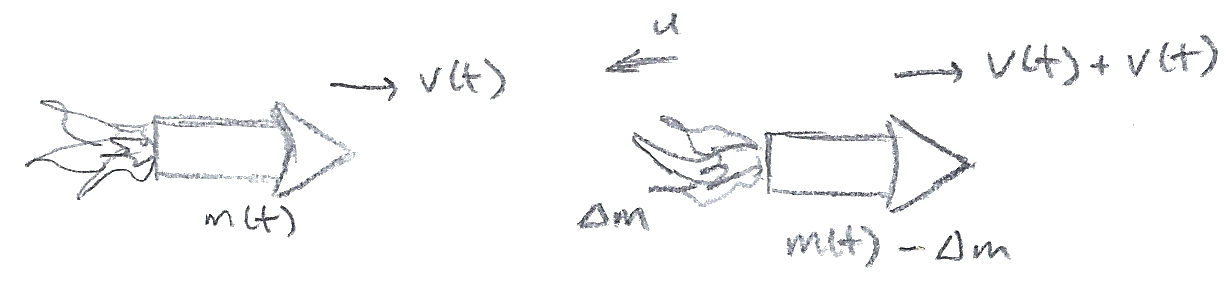
\includegraphics[width=0.5\textwidth]{images/mechintro/rockets.png}\\
\end{center}
To set this up, let $m(t)$ be the mass of the rocket as a function of time, $v(t)$ be the velocity (in one dimension, for simplicity) and $u$ be the exhaust velocity, or how fast the mass being shot out the back end is going. \\
Since we're assuming no external forces are acting on the system, we can apply conservation of linear momentum. At some time $t$, we know the magnitude of the momentum of the rocket, $P^{tot}$:
\[
	P^{tot}_i = m(t) v(t) 
\]
Now, after a time $\Delta t$, we know the rocket has changed by a mass $\Delta m$ (which is negative) and increased its speed by $\Delta v$. Relative to the rocket, the exhaust is being jettisoned backwards at a velocity of $-u$, but relative to the reference frame, since the rocket is moving at a velocity of $v(t) + \Delta v$, the exhaust is moving at a velocity $v(t) + \Delta v - u$. From this, we can calculate the magnitude of the total linear momentum after a small time interval:
\[
	P^{tot}_f = (m(t) + \Delta m)(v(t) + \Delta v) - \Delta m (v(t) + \Delta v - u)
\]
This looks a bit messy, but we can condense it to the following: 
\[
	P^{tot}_f = m(t)v(t) + m(t) \Delta v + \Delta m u 
\]
By conservation of linear momentum, $P^{tot}_i = P^{tot}_f$, so canceling $m(t)v(t)$ we have that:
\[
	m(t) \Delta v = - \Delta m u
\]
One final step: as the length of the time interval we observe $\Delta t$ goes to $0$, we want to consider the rate of change of the velocity and mass, so we will reformulate this in terms of derivatives:
\[
	m(t) \dv{v}{t} = - \dv{m}{t} u
\]
This is the rocket equation. The term on the right-hand side is defined as the thrust of the rocket. However, if we'd like to know an actual function that models the motion of the rocket, this isn't quite enough. We're going to solve our first differential equation to find the velocity of the rocket and its relation to the mass of the rocket over time. \\
Let's rearrange this as follows: 
\[
	\frac{1}{u} \dv{v}{t} = - \frac{1}{m(t)} \dv{m}{t} 
\]
Let's integrate both sides with respect to time from time $t=0$ to some arbitrary time $t$:
\[
	\int_0^t \frac{1}{u} \dv{v}{t} \, dt = - \int_0^t \frac{1}{m(t)} \dv{m}{t} \, dt 
\]
\[
	\int_0^t \dv{}{t}\left(\frac{v}{u}\right) \, dt = - \int_0^t \dv{}{t} \left(\ln m(t) \right) \, dt
\]
\[
	\frac{v(t)}{u} - \frac{v_0}{u} = \ln m_0 - \ln m(t) 
\]
To simplify even further, let's just assume the rocket starts from rest, so we end up with a final result of:
\[
	v(t) = u \ln \frac{m_0}{m(t)}
\]
where $m_0$ is the initial mass of the rocket. \\
A little bit of fiddling with this reveals why rockets have to carry so much fuel: in order to maximize the velocity rockets have to be able to shoot out fuel at top speeds, and burn up a lot of their mass in order to get to fast enough speeds to escape Earth's gravity. \\
A small sidenote - letting $u$ be arbitrarily large creates problems not only practically, but also in theory: as $u$ approaches the speed of light, this model will give us velocities that are way over that speed - but the speed of light turns out to be a "speed limit" on the universe - nothing can travel faster than that. So there's something wrong with one of our assumptions somewhere! It turns out the correct expression for momentum isn't what we think it is at large speeds, but works for small speeds well enough - we'll discuss this if we talk about special relativity. 
\subsubsection{Summary and Problems}
Linear momentum is a good quantity to keep track of, especially when no outside forces are acting on the system like during a collision or explosion, in order to see how objects in the system move. We also learned how to calculate use the center of mass of an object to properly see how forces can impact the trajectory of the object, even if the situation is too computationally intensive to know the full motion of the block. \\

\noindent \textbf{Problems}\\
1. (2 $\bigstar$) A bullet with mass $m_1$ moving directly upward with speed $v_i$ strikes and passes through the center of mass of a block with mass $m_2$ which is initially at rest. The bullet emerges from the block moving directly upward and has slowed to a speed $v_f$. Show that the maximum height $h$ that the block rises above its initial position is $h = \frac{m_1^2 (v_i-v_f)^2}{2gm_2^2}$.\\
2. (1 $\bigstar$) A vessel at rest at the origin of an $xy$-coordinate system explodes into three pieces. Just after the explosion, one piece, of mass $m$, moves with velocity $v$ in the $-x$-direction and a second piece, also of mass $m$, moves with velocity the same magnitude in the $-y$-direction. The third piece has mass $3m$. Just after the explosion, show that the magnitude and direction of the velocity of the third piece is $\frac{\sqrt{2}}{3}$ with a direction of $45$ degrees counterclockwise from the $+x$-axis.\\
3. (3 $\bigstar$) A block of mass $m_B$ falls vertically through a height $h$ and then collides with a pile of mass $m_P$, driving it a distance $\Delta y$ into bedrock. Assuming that the block-pile collision is completely inelastic, show the magnitude of the average force on the pile from the bedrock during the descent of $\Delta y$ is $F = \frac{m_B^2hg}{\Delta y(m_B+m_P)}$.\\
4. (2 $\bigstar$, $\spadesuit$) A long, thin wire of length $L$ has a density given by $A-Bx$, where $A$ and $B$ are positive constants and $x$ is the distance from the more massive end. Show that the center of mass of the rod is at $x_{COM} = \frac{\frac{1}{2}AL-\frac{1}{3}BL^2}{A-\frac{1}{2}BL}$.\\
5. (4 $\bigstar$) A stream of elastic glass beads, each with a mass $m$, comes out of a horizontal tube at a rate of $n$ per second. The beads fall a distance of $d$ to a balance pan and bounce back to their original height. Show that the mass that must be placed in the other pan of the balance to keep it balanced is $2mn\sqrt{\frac{2d}{g}}$.\\
6. (3 $\bigstar$) A car with mass $m$ sits initially at rest on top of a long horizontal platform of mass $3m$ and length $L$. The platform rests on a horizontal surface with negligible friction between the platform and the horizontal surface. The platform and the car have zero velocity with respect to the horizontal surface at time $t=0$. The car begins to move with constant acceleration of magnitude $A$ with respect to the platform in the $+x$-direction (rightward) at time $t=0$. It continues to move at constant acceleration until it reaches the end of the platform. Show that the velocities of the car and platform with respect to the horizontal surface are $\frac{3\sqrt{2LA}}{4} \hat x$ and $-\frac{\sqrt{2LA}}{4} \hat x$, respectively.\\ 
7. (4 $\bigstar$, $\spadesuit$) A rocket in space moves in a straight line from rest with initial mass $m_0$. The rocket burns fuel at a non-constant rate but ejects the fuel at a constant speed relative to the rocket $u$. The rate of burning fuel is adjusted so that the rocket accelerates at a constant rate of $g$. Show that the mass of the rocket $m(t)$ can be modeled as $m(t) = m_0 e^{-gt/u}$, and the time it takes for the rocket to be reduced to 1\% of the original mass is $\frac{u}{g}\ln(100)$.

\pagebreak

\subsection{Rotation and Angular Momentum}
From up until this point, we've been dealing in translational motion, where objects move physically from place to place. We're going to reformulate what we've done so far for bodies that only rotate in place, and build up to another conservation law - conservation of angular momentum, the rotational analog to linear momentum. 
\subsubsection{Rotational Kinematics}
When we talk about rotation, we already have the tools to generate kinematic equations for rotation. Instead of position, we have the angle $\theta$ that a body has turned with respect to an axis (which is a unitless scalar quantity). The angular velocity $\omega$ is the time-derivative of the angle $\theta$, similar to the velocity we already know, and angular acceleration $\alpha$ for the time-derivative of the angular velocity, similar to our regular acceleration. Using the same derivations as before for our constant-acceleration kinematic equations, we attain the following: 
\[
	\omega^2 - \omega_0^2 = 2\alpha\Delta\theta
\]
\[
	\theta(t) = \theta_0 + \omega_0 t + \frac{1}{2} \alpha t^2 
\]
One subtlety to note: In three dimensions, which we will soon be using on a regular basis for rotation, angular velocity and acceleration are both vectors that point perpendicular to the velocity and position vectors. Their direction is more specifically specified using the right-hand-rule: that is, as you curl your hand in the direction of the rotation, the thumb should point in the direction of the angular velocity. In fact, we can use the vector cross product to define these vector quantities: 
\[
	\vec v = \vec \omega \times \vec r
\]
\[
	\vec a = \vec \omega \times \vec v + \vec \alpha \times \vec r
\]
These should look somewhat like the formulas we saw for circular motion. The formula for velocity is about the same, just a bit more general if the velocity and position are not perfectly perpendicular to each other. The same is true for the acceleration, where we have that the first term is the centripetal acceleration while the second term is the tangential acceleration. Get comfortable using your right hand. You will see cross products often going forward. 
\subsubsection{Moment of Inertia and Torque}
After considering a rotational analogue for kinematics, we now turn to find a rotational way of describing dynamical systems. To do this, we use the concept of torque on a point particle with respect to a point: 
\[
	\vec \tau = \vec r \times \vec F
\]
where $\vec \tau$ represents the torque on the particle with respect to some point, $\vec r$ the position vector from this arbitrary point to the position of the point particle, and $\vec F$ the net force on that particle. Note that we can use Newton's Second Law, $\vec F = m\vec a$, to substitute in for the force. We can resolve the acceleration into tangential and centripetal components, so we have: 
\begin{align*}
	\vec \tau &= \vec r \times (m \vec a) \\
	&= m \vec r \times (\vec a_c + \vec a_t) \\
	&= m (\vec r \times \vec a_c + \vec r \times \vec a_t) 
\end{align*}
However, since the centripetal acceleration and position vector point in the same direction, their cross product is $0$. For the tangential acceleration, we have $\vec a_t = \vec \alpha \times \vec r$. We can then write the torque as:
\[
	\vec \tau = m \vec r \times \vec alpha \times \vec r
\] 
We can use an expansion of the vector triple product, where $\vec A \times \vec B \times \vec C = \vec B(\vec A \cdot \vec C) - \vec C(\vec A \cdot \vec B)$. Then, we have:
\[
	\vec \tau = m(\vec \alpha (\vec r \cdot \vec r) - \vec r(\vec \alpha \cdot \vec r))
\] 
Noting $\vec \alpha \cdot \vec r = 0$ as $\vec \alpha$ is perpendicular to the plane of rotation, we have:
\[
	\vec \tau = mr^2 \vec \alpha
\]
where $r$ is the distance away from the reference point. For an entire body, we can add up all of these individual torques, noting that the angular acceleration for a rigid body is the same throughout:
\[
	\sum \vec \tau = \sum_i m_i r_i^2 \vec \alpha = I \vec \alpha
\]
This is Newton's Second Law for Rotation. This sum that appears on the right-hand side is called the moment of inertia, denoted $I$, and is taken with respect to an axis of rotation. (For sufficiently symmetric systems, even though we're taking the torque with respect to a point, it can be shown that taking the torque with respect to the entire axis of rotation is equivalent. We'll discuss this when looking at angular momentum.) \\
For discrete systems of point particles, the sum 
\[
	I = \sum_i m_i r_i^2
\]	
for a rigid body is enough to calculate the moment of inertia. However, for large rigid bodies we have to integrate, similar as we did for the center of mass:
\[
	I = \int r^2 \, dm
\]
where $r$ refers to the distance each infinitesimally small part $dm$ is from the reference point. \\
As an example, we'll do a uniform spherical shell with radius $R$ and mass $M$. The surface density $\sigma$ will then just be the mass per unit area, so $\sigma = \frac{M}{4\pi R^2}$. For this 3-D object, let the $y$-axis (directly upward) be the axis of rotation that we're calculating the moment of inertia about. This is a pretty tricky example, which can be done by splitting this shell into rings perpendicular to the axis of rotation. Let $\theta$ be the angle between the positive $y$-axis and the line joining the edge of the ring to the center. This angle ranges from $0$ to $\pi$. \\
\begin{center}
	\begin{asy}
		import solids;
        import three;
        size(7cm);
        real theta = 40;
        currentprojection=orthographic(0.7, -4, 1);
        currentlight=nolight;
        triple center = (0,0,0);
        triple ringctr = (0, 0, Cos(theta));
        real R=1, RS=0.7, inc=100, lat=45, lon=45, tlat=50, tlon=100;
        dot(center);
        real r = 2;
        dot(ringctr);
        revolution Earth=sphere(center, R);  
        triple contact = (Sin(theta), 0, Cos(theta));
        
        draw(surface(Earth), surfacepen=white+opacity(.1), meshpen=0.7*black);
        draw(arc(ringctr, Sin(theta), 90, 180, 90, 0), linewidth(2));
        draw(arc(ringctr, Sin(theta), 90, 0, 90, 180), linewidth(2)+linetype("4 4"));
        draw(center--(Sin(theta), 0, Cos(theta)));
        draw(center--(0,0,R));
        draw(ringctr--contact);
        
        label("$R$", (Sin(theta)/2, 0, Cos(theta)/2), dir(360-theta));
        label("$dM$", contact, dir(40)*1.5);
        label("$\theta$", center, dir(90-(theta/2))*3);
        label("$R \sin\theta$", (Sin(theta)/2, 0, Cos(theta)), dir(90));
	\end{asy}
\end{center}
Now, we need to calculate $dm$ in terms of $\theta$. For any $\theta$, the set of all points on the shell that make an angle of $\theta$ between a radius of that point and the positive $y$-axis is a ring with radius $R\sin \theta$. This ring has "thickness" $R \, d\theta$, which is the length of the arc spanned by a small change $d\theta$ and has a circumference $2 \pi R \sin \theta$. Therefore, the surface area of the ring is $2 \pi R^2 \sin \theta \, d\theta$, and then the mass of the ring is this expression times the surface density, $\sigma$. This gives $dm = 2 \sigma \pi R^2 \sin \theta \, d\theta$. Since the distance from the edge of each ring to the axis is just the radius of each ring, $R \sin \theta$, we can now evaluate the integral:
\begin{align*}
	I &= \int_0^\pi (R \sin \theta)^2 \, dm \\
	&= \int_0^\pi R^2 \sin^2 \theta \cdot 2 \sigma \pi R^2 \sin \theta \, d\theta \\
	&= 2\pi \sigma R^4 \int_0^\pi \sin^3 \theta \, d\theta\\
	&= 2\pi \sigma R^4 \int_{-1}^1 1 - u^2 \, du \\
	&= 2\pi \sigma R^4 \left( u - \frac{1}{3}u^3 \Big|_{-1}^1 \right)	\\
	&= 2 \pi\frac{M}{4\pi R^2}  R^4 \frac{4}{3} = \frac{2}{3}MR^2
\end{align*}
This is a pretty hard example - the trigonometric integral is dealt with by using $\sin^2 \theta = 1 - \cos^2 \theta$ and then substituting $u = \cos \theta$. Also, the setup of $dm$ is hard - one has to realize the "thickness" of the ring not only exists, but also is along the surface of the sphere rather than straight up and down. Calculations don't really get much harder than this, and all the required moments of inertia to know can be derived using a one-dimensional integral. (The most common ones are included as an appendix.)\\
One final thing about moments of inertia: for most cases, such as the sphere we just derived, the axis of rotation will pass through the center of mass, making the derivation for the moment of inertia fairly straightforward. However, there are cases where we will need the axis of rotation to not pass through the center of mass, but through some parallel axis. We can use the aptly-named Parallel Axis Theorem to help with this, which states:
\[
	I_{cm} + Mh^2 = I
\]
where $I$ is the moment of inertia about an axis through some point, $h$ the distance between that point and the center of mass, $M$ the total mass, and $I_{cm}$ the moment of inertia about an axis through the center of mass. The proof of this can be done using calculus, but we will prove it later using energy. 
\subsubsection{Angular Momentum}
Angular momentum is the rotational analog of momentum, defined as follows for a point particle and denoted with the vector $\vec L$:
\[
	\vec L = \vec r \times \vec P
\]
where $\vec r$ is the position of the point particle with respect to some arbitrary point. 
We can take a time derivative of this expression to attain a familiar-looking expression:
\[
	\dv{\vec L}{t} = \dv{}{t}(\vec r \times \vec P) = \dv{\vec r}{t} \times \vec P + \vec r \times \dv{\vec P}{t} = \vec v \times m\vec v + \vec r \times \vec F = \vec r \times \vec F = \vec \tau
\]
The angular momentum of a particle with respect to a point, then, follows all the same rules that linear momentum follows with forces. First, we can now imagine torques as the flow of angular momentum being delivered to and from objects. The angular impulse delivered to a system, then, can be shown to be the change in angular momentum - this is the angular version of the impulse-momentum theorem: 
\[
	\Delta \vec L = \int_{t_1}^{t_2} \vec \tau \, dt
\]
Also, for a system of particles, the time derivative of the total angular momentum of a system of particles with respect to a point is the net external torque on the system:
\[
	\vec \tau_{net} = \dv{\vec L_{sys}}{t}
\]
This can be shown using the same techniques as before with careful consideration of internal and external torques. When no external torques are acting on the system, we know that $\vec L$ is a constant, which gives us the principle of conservation of angular momentum, similar to that for linear momentum: 
\begin{mdframed}[frametitle=Conservation of Angular Momentum]
For a system with no external torques, angular momentum is conserved - the total amount of angular momentum in the system remains constant and is not changed by the internal motion/dynamics of the system.
\end{mdframed}
We'd now like to be able to relate angular momentum to the motion of the center of mass. For a rigid body, the total angular momentum of that object with respect to some arbitrary point is the sum of the angular momenta for each particle within:
\[
	\vec L^{tot} = \sum_i \vec L_i = \sum_i \vec r_i \times \vec P_i = \sum_i \vec r_i \times m_i \vec v_i
\]
where the $\vec r_i$ are the positions of each particle with respect to this arbitrary point, the $\vec v_i$ each particle's velocity, and $m_i$ the mass. \\
Let's force the center of mass into the expression by expressing each position and velocity vector of each particle as the sum of the position/velocity of the center of mass and its position/velocity relative to the center of mass (henceforth referred to as $\vec r_i^*$ and $\vec v_i^*$). Let's plug it all in and distribute the terms:
\begin{align*}
	\vec L^{tot} &= \sum_i (\vec r_{cm} + \vec r_i^*) \times m_i(\vec v_{cm} + \vec v_i^*) \\
	&= \sum_i \vec r_{cm} \times m_i \vec v_{cm} + \sum_i \vec r_{cm} \times m_i \vec v_i^* + \sum_i \vec r_i^* \times m_i \vec v_{cm} + \sum_i \vec r_i^* \times m_i \vec v_i^* 
\end{align*}
These sums all look pretty bad. Let's just take them one at a time. \\
For the first sum, we notice that we can more or less factor out the cross product, and be left with: 
\[
	\sum_i \vec r_{cm} \times m_i \vec v_{cm} = \vec r_{cm} \times \vec v_{cm} \left(\sum_i m_i \right) = \vec r_{cm} \times M\vec v_{cm} = \vec r_{cm} \times \vec P^{tot}
\]
where the total mass of the object is $M$. \\
The second and third sums I claim to be $\vec 0$. This is very tricky to see, but we'll look at the second sum first. First, we can use the fact that the cross product distributes over addition to rearrange the sum, and then we can examine what's left more closely:
\[
	\sum_i \vec r_{cm} \times m_i \vec v_i^*  = \vec r_{cm} \times \sum_i  m_i \vec v_i^*
\]
Where have we seen something similar to this sum before? This looks like the expression for the velocity of the center of mass of an object with respect to some reference point, up to a factor of $M$. However, our reference point IS the center of mass, so this clearly then comes out to be the zero vector. Therefore, 
\[
	\vec r_{cm} \times \sum_i  m_i \vec v_i^* = \vec r_{cm} \times M\vec 0 = \vec 0
\]
Similarly, the sum that appears after rearranging the third sum is the position of the center of mass with respect to the center of mass, which also is the zero vector:
\[
	\sum_i \vec r_i^* \times m_i \vec v_{cm} = \sum_i m_i \vec r_i^* \times \vec v_{cm} = M\vec 0 \times \vec v_{cm} = \vec 0 
\]
The last part is the trickiest part to evaluate. For this, we use the fact that $\vec v_i^* = \vec \omega \times \vec r_i^*$ and $\vec \omega$ is both constant for each particle in the rigid body and perpendicular to the plane that the particle rotates in, as the body rotates about its center of mass: 
\[
	\sum_i \vec r_i^* \times m_i \vec v_i^* = \sum_i m_i (\vec r_i^* \times \vec \omega \times \vec r_i^*) = \sum_i m_i \left[ \vec \omega \left(r_i^*\right)^2 - \vec r_i^*(\vec r_i^* \cdot \vec \omega) \right]  = \sum_i m_i \left(r_i^*\right)^2 \vec \omega
\]
That sum has an expression for the moment of inertia of the rigid body, with respect to its center of mass in it! This now is cleanly written as:
\[
	\sum_i \vec r_i^* \times m_i \vec v_i^* = I_{cm}\vec \omega
\]
So, altogether: 
\[
	\vec L^{tot} = \vec r_{cm} \times \vec P^{tot} + I_{cm} \vec \omega = \vec L^{orb} + \vec L^{spin} 
\]
The first term with the cross product is called the orbital angular momentum (considering how much the object is revolving about the reference point), and the second term is the spin angular momentum (considering how much the object is spinning about its center of mass). Usually, we will pick the reference point so that one of these two terms is zero, more likely than not making the orbital angular momentum zero. For the most part:
\[
	\vec L^{tot} = I_{cm} \vec \omega 
\]
One subtlety is that we normally don't consider angular momentum about a point, but rather an axis of rotation - what we mean by this is that the angular momentum is the same for any point on the axis. This is only true for objects with cylindrical or spherical symmetry, which is sufficient for what we are using it for, but not in the general case. 
\subsubsection{Statics and Rolling Without Slipping}
Armed with the knowledge of rotation, we can look at dynamical systems that are not only moving in space but also rotating. One of the easiest cases is that for systems that are completely at rest, or in a state of static equilibrium. This means that there is no net force on the system, and no net torque. To approach these problems, we will draw extended free-body diagrams, which not only list all of the forces but also show where they act in relation to each other in order to help compute torques. Even though we've seen some statics problems before when discussing forces, be careful to also account for all torques due to gravity (acting at the center of mass) and the torques from contact forces.\\
As an example, consider a long, thin beam of mass $M$ and length $L$, fixed to a vertical wall at a pivot point and at an angle of $\theta$ below the horizontal. An ideal string tied at the end of the beam holds it up, and this string is fixed vertically upwards to the ceiling. We want to find the tension in the string. \\
\begin{center}
	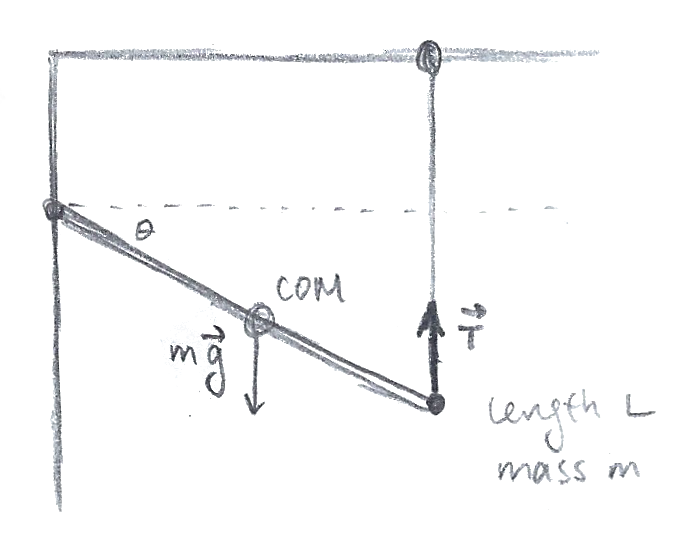
\includegraphics[width=0.4\textwidth]{images/mechintro/statics.png}\\
\end{center}
At first, it seems tempting to just apply Newton's Second Law for all the contact forces and gravity, but quickly it becomes clear that we don't really know how the force from the pivot point really works, and we're missing this information to solve the problem. It's actually much easier to consider the sum of the torques about the pivot point. Since the center of mass of the beam is at the halfway point, the torque due to gravity has magnitude $\tau_g = \frac{L}{2}Mg\cos \theta$. (Make sure you understand why it's cosine and not sine - it's because of the angle between the vectors.) The forces all lie in the same plane, so all the torques run in and out of the page. If we consider up to be the $+y$-direction, right to be the $+x$-direction, and out of the page to be the $+z$-direction (since $\hat x \times \hat y = \hat z$), we have: 
\[
	\sum \tau_z = -\frac{MgL\cos \theta}{2} + \tau_{string} = 0
\]
Therefore, we have that the torque from the string (in the $z$-direction is $\tau_{string} = \frac{MgL\cos \theta}{2}$, since no net torque acts on the system. Noting that $\tau_{string} = TL\cos \theta$, where $T$ is the tension, from this, we can see that the tension $T = \frac{Mg}{2}$. \\
Frequently, aside from using kinematics to look at the system, sometimes we are given that some object or another is rolling without slipping. This means that the following two are true, for a circular object of radius $R$: 
\[
	v_{cm} = \omega R \quad a_{cm} = \alpha R
\]
\begin{center}
	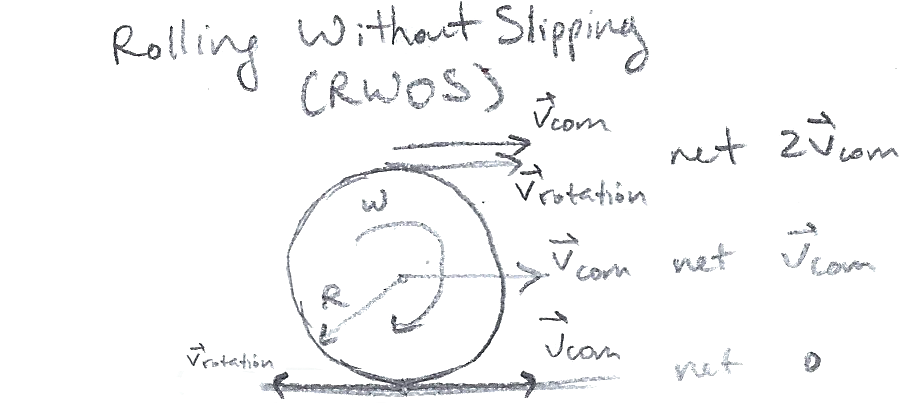
\includegraphics[width=0.4\textwidth]{images/mechintro/rwos.png}\\
\end{center}
When this is true, the frictional force that the object encounters with the ground is actually static and does not change the acceleration of the object. If the object's velocity/angular velocity, etc. do not satisfy these relations, the force of friction will either speed up or slow down the object in order for these two to match so the object starts to roll without slipping. You can see this the next time you go bowling - when you release the ball, the ball slides with constant velocity, but friction begins to turn the ball and it begins to spin faster, and eventually roll normally as the ball travels down the alley. \\
A consequence of the above relations is that relative to the ground, the point in contact with the ground has zero velocity relative to the ground, and the top of the object has speed $2v_{cm}$ relative to the ground. This is very useful to know sometimes - and it can be shown using the principles of relative motion that we discussed in kinematics. \\
Let's revisit Atwood's machine to see how rolling without slipping affects the situation. Consider two masses of $m_1$ and $m_2$ both attached to a taut string ($m_2 > m_1$), wrapped around a solid cylindrical pulley of mass $m_p$ and radius $R$ that is free to spin about its axis. The string does not slip on the pulley, and is still effectively massless. \\
\begin{center}
	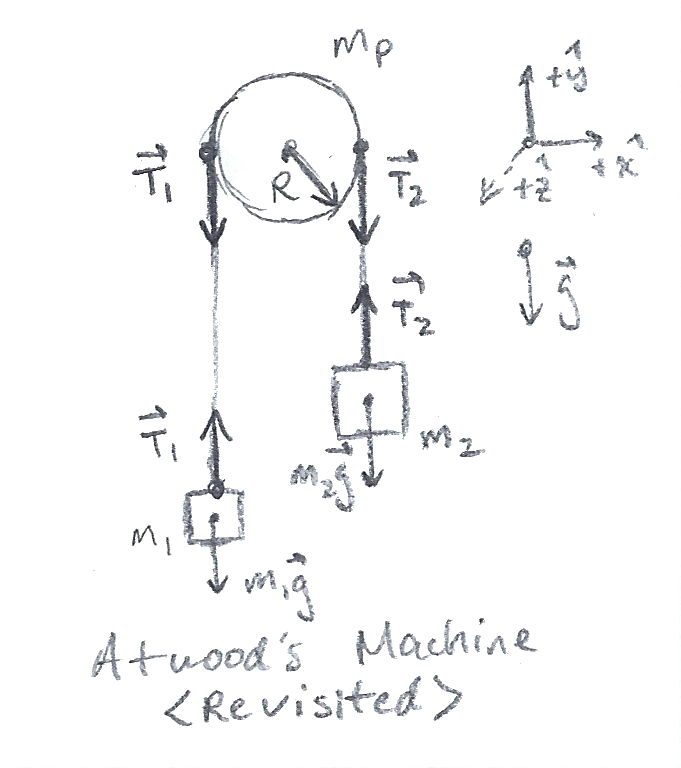
\includegraphics[width=0.4\textwidth]{images/mechintro/atwood-revisited.png}\\
\end{center}
We've drawn an extended free-body diagram to show where each force acts in relation to the objects in the diagram. Notice that the tensions in the strings connecting $m_1$ and $m_2$ to the pulley are not the same, because they're connected to a rotating body now. To distinguish them, let's label the tension on $m_1$ as $T_1$ and the tension on $m_2$ as $T_2$. Let's set up Newton's Second Law, taking into account the force on each of the blocks as well as the torque on the pulley:
\[
	\sum_1 \vec F_i = m_1 \vec g + \vec T_1 = m_1 \vec a
\]
\[
	\sum_2 \vec F_i = m_2 \vec g + \vec T_2 = -m_2 \vec a
\]
\[
	\sum_p \vec \tau_i = \vec R \times \vec T_1 + \vec R \times \vec T_2 = I \vec \alpha
\]
We can project the components of the force in the $+y$-direction (up and down the page), and project the components of the torque along the $+z$-direction (in and out of the page), to get:
\[
	\sum_1 F_y = -m_1g + T_1 = m_1a 
\]
\[
	\sum_2 F_y = -m_2g + T_2 = -m_2a
\]
\[
	\sum_p \tau_z = RT_1 - RT_2 = -I\alpha = -\frac{1}{2}m_pR^2 \alpha
\]
Notice how the sign of the acceleration is reversed for the second block, since we know it's going downwards. Similarly, we've placed a negative sign in front of the angular acceleration since the pulley is rotating clockwise. However, we only have three equations, but we now have four unknowns - the two tensions, the angular acceleration of the pulley, and the acceleration of the blocks. The final thing we need to invoke is the no-slipping condition, which implies the following relation between the angular acceleration of the pulley and the blocks:
\[
	a = R \alpha
\]
We now have all the information we need to solve for the acceleration of the blocks, and the two tensions. Omitting the messy algebra, we have:
\[
	a = \frac{m_2-m_1}{m_1+m_2+\frac{1}{2}m_p}g \quad T_1 = m_1g\frac{4m_2+m_p}{2m_1+2m_2+m_p} \quad T_2 = m_2g\frac{4m_1+m_p}{2m_1+2m_2+m_p} 
\]
Clearly, these expressions are very different than the ones we saw earlier for Atwood's machine, since they now all involve the mass of the pulley from the pulley's moment of inertia.\\
Rolling without slipping problems are a bit more complex, and usually, some information might seem to be missing from the problem in order to solve them. After all, you need to have the same number of variables as equations in order to solve them. If you seem to be missing an equation, it's not a bad idea to impose the rolling without slipping condition on the situation to see if the situation is solvable then. \\
\subsubsection{Summary and Problems}
We now have the tools to look at dynamical systems from a rotational perspective as well as from a translational one. In the following problems, be sure to account for both of these and be able to relate the two different systems of dynamics to each other, with an emphasis on torques, moments of inertia, and angular momentum. \\

\noindent \textbf{Problems}\\
1. (1 $\bigstar$) A uniform cylinder of mass $M$ and radius $R$ has a string wrapped around it. The string is held fixed, and the cylinder falls vertically. a) Show the acceleration of the cylinder is downward with magnitude $a = \frac{2g}{3}$. b) Show the tension in the string $T = \frac{Mg}{3}$. \\
2. (2 $\bigstar$) A uniform solid cylinder of mass $M$ and radius $R$ is at rest on a slab of mass $m$, which in turn rests on a horizontal, frictionless table. If a horizontal force is applied to the slab, it accelerates and the cylinder rolls without slipping. Show the acceleration of the slab is $a = \frac{3F}{3m+M}$.\\
3. (3 $\bigstar$, $\spadesuit$) A uniform horizontal disk of mass $M$ and radius $R$ is spinning about the vertical axis through its center with an angular speed $\omega$. When the spinning disk is dropped onto a horizontal tabletop, kinetic-frictional forces on the disk oppose its spinning motion. Let $\mu_k$ be the coefficient of kinetic friction between the disk and the tabletop. Show that the time required for the disk to stop rotating is $\Delta t = \frac{3R\omega}{4\mu_kg}$. Hint: First, compute the total torque on the disk (from where?) by dividing the disk into thin rings and computing the torque on each ring. \\
4. (2 $\bigstar$) A particle that has a mass $m$ is traveling with a constant velocity along a straight line that is a distance $b$ from the origin $O$. Let $dA$ be the area swept out by the position vector from $O$ to the particle during a time interval $dt$. Show that $\dv{A}{t}$ is constant and is equal to $\frac{L}{2m}$, where $L$ is the magnitude of the angular momentum of the particle about the origin. \\
5. (3 $\bigstar$) A uniform solid sphere with mass $M$ and radius $R$ is set rotating about a horizontal axis at an angular speed $\omega_0$ and then is placed on the floor with its center of mass at rest. If the coefficient of kinetic friction between the sphere and the floor is $\mu_k$ show the speed of the center of mass of the sphere $v = \frac{2R\omega_0}{7}$ when the sphere begins to roll without slipping. \\
6. (4 $\bigstar$) A uniform ladder of length $L$ and mass $m$ leans against a frictionless vertical wall, making an angle of $\theta$ with the horizontal. The coefficient of static friction between the ladder and the ground is $\mu_s$. If your mass is $k$ times that of the ladder, show that the maximum displacement you can move along the ladder $r$ is given by $r = \mu_s L\tan\theta\left(1 + \frac{1}{k}\right) - \frac{L}{2k}$. \\
7. (4 $\bigstar$) A block of mass $M$ rests on a table, connected by a string to a cylindrical (NOT FIXED) pulley of mass $M$ and radius $R$. The string wraps around the pulley and is tied to a block of mass $M$ dangling over the edge of the table. The coefficient of static and kinetic friction between the block on the table and the table is $\frac{1}{2}$. When the system begins moving, the string moves on the cylinder without slipping. Show that the acceleration of each of the blocks is $a = g/5$, and the tensions in the strings are $\frac{4}{5}Mg$ in the string holding the hanging block, and $\frac{7}{10}Mg$ in the string pulling the block along. 
\pagebreak

\subsection{Energy}
The final conserved quantity that we will use to analyze problems is energy. It is the only scalar that we are looking at that is conserved, and is always a positive number. Energy is measured in joules (J), and by definition 1 J = 1 N $\cdot$ m = kg $\cdot$ m$^2$/s$^2$. The rate at which energy is transferred is power and has units of watts (1 W = 1 J/s). 
\subsubsection{Work and Kinetic Energy}
Work is the transfer of energy between objects, and a force is said to do work if the object it is acting upon is displaced, and we might remember it's force times distance - but we need a better definition for work. 
\begin{center}
	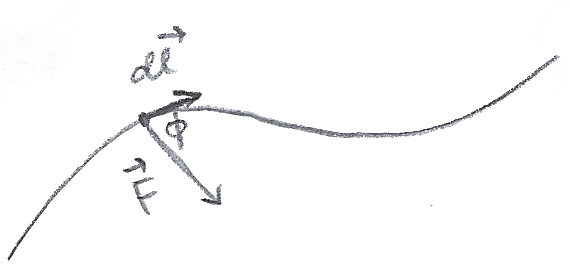
\includegraphics[width=0.3\textwidth]{images/mechintro/work.png}\\
\end{center}
As an object moves along a path while being acted upon by a force, we can split the path into many small displacements. Since work serves to set objects into motion, only the component of the force in the direction of the displacement counts towards the work. So, if the displacement is $d \vec l$, and $\vec F$ is the force, the component of the force in the direction of the displacement is $F \cos \phi$ if $\phi$ is the angle between the displacement and the displacement. This can be written as $\vec F \cdot d\vec l$. Therefore:
\[
	dW = \vec F \cdot d\vec l
\]
where $W$ is the work. For constant force $\vec F$ and linear displacement $d \vec l$ this is true, but to find the total work along any curve $C$, we can let all the little displacements go to zero, let the number of displacements go to infinity and add up all of the little components of work. This is an integral, but a type of integral that we won't encounter in BC Calculus. Somewhat fittingly, this kind of integral is called a line integral, and we can write it as follows:
\[
	W = \int_C \vec F \cdot d\vec l
\]
We won't have to evaluate general line integrals, but for relatively simple cases we will (where the distance is basically linear). \\
This expression for work seems very niche, but we can construct such a line integral from Newton's Second Law, $\vec F = m\vec a = m \dv{\vec v}{t}$. First, we dot the vector on both sides with $\vec v$:
\[
	\vec F \cdot \vec v = m \vec v \cdot \dv{\vec v}{t}
\]
Now, we can integrate with respect to $t$ between times $t_1$ and $t_2$:
\[
	\int_{t_1}^{t_2} \vec F \cdot \vec v \, dt = \int_{t_1}^{t_2} m \vec v \cdot \dv{\vec v}{t} \, dt
\]
The dot product follows the product rule, so I claim that $\frac{1}{2} \dv{}{t}\vec v \cdot \vec v = \vec v \cdot \dv{\vec v}{t}$. Indeed, $\frac{1}{2} \dv{}{t}\vec v \cdot \vec v = \frac{1}{2} \left( \dv{\vec v}{t} \cdot \vec v + \vec v \cdot \dv{\vec v}{t} \right) = \vec v \cdot \dv{\vec v}{t}$. Therefore:
\[
	\int_{t_1}^{t_2} \vec F \cdot \vec v \, dt = \int_{t_1}^{t_2} \frac{1}{2} m \dv{}{t}\vec v \cdot \vec v \, dt = \frac{1}{2} m (\vec v(t_2) \cdot \vec v(t_2) - \vec v(t_1) \cdot \vec v(t_1)) = \frac{1}{2}m (v_{t_2}^2 - v_{t_1}^2 )
\]
The quantity $\frac{1}{2} mv^2$ one might recognize as the kinetic energy $K$ of an object with mass $m$ and velocity $v$, from chemistry. As a refresher, the kinetic energy of an object is the energy the object has that is stored in its movement. This right hand side describes the change in the kinetic energy as the velocity of the object changes during the time interval, so we can write it as $\Delta K$. On the left hand side, since $\dv{\vec l}{t} = \vec v$, $d\vec l = \vec v \, dt$, so we can write the left hand side as an integral along the curve followed by the object during the time interval. In other words, it's our line integral for work! Therefore:
\[
	W = \int_C \vec F \cdot d\vec l = \Delta K
\]
This is the Work-Energy Theorem, which is useful for determining how much work is done to an object after a process by instead measuring its kinetic energy at the beginning and end of the process. \\
As a final sidenote, it's worth noting that kinetic energy has both a translational and rotational form. For an object, a body has translational kinetic energy of $\frac{1}{2}mv^2$, but rotational kinetic energy $\frac{1}{2}I\omega^2$. This expression pops up in the same way when torque is dotted with the angular velocity. Always remember to account for rotational kinetic energy when dealing with rotating objects as well!
\subsubsection{Potential Energy}
Before we introduce the other kind of mechanical energy we'll be studying, potential energy, we have to first introduce the idea of conservative forces versus non-conservative forces. Let's look back at the formula for work: 
\[
	W = \int_C \vec F \cdot d\vec l
\]
For a force $\vec F$, if the work done on the object is independent of the path the object travels, then $\vec F$ is said to be a conservative force. If $\vec F$ does not satisfy this, it is non-conservative. Notice that for $\vec F$ to be conservative, we must have that the work done on an object around a closed loop is zero. Symbolically:
\[
	W = \oint_C \vec F \cdot d\vec l = 0
\]
where the symbol $\oint$ represents integrating around a closed loop (but it's still a line integral). This can be seen by noting that as a particle moves by a conservative force from point $A$ to point $B$, doing some amount of work, the exact negative work is done as the particle moves back from point $B$ to point $A$. With this, we can define the potential energy function $U$ - as work is applied to an object, the potential energy of the object should decrease by the same amount:
\[
	\Delta U = - \int_C \vec F \cdot d\vec l = - W
\]
Usually, potential energy functions are dependent upon the position of the object with respect to the conservative forces at play and give a scalar energy to every point in space, but we'll really only deal with functions in one dimension. The concept is still the same. Also, usually when integrating we'll get a constant - but to simplify things we'll set it to zero, which will sometimes produce negative values of potential energy - but that's fine because it's the relative differences between values that matter more than the actual values. To illustrate this, we'll use an arbitrary one-dimensional conservative force, and look at the potential energy of a particle being acted upon by this force:
\[
	F_x = F_0 \cos \left(\frac{2\pi x}{L} \right)
\]
For the sake of simplicity, both $F_0$ and $L$ have the correct dimensions of force and length, respectively and are both positive.\\ First, let's try to find the potential energy. Consider a path from $x = 0$ to arbitrary $x$ along a straight line. When we do this line integral, then, the dot product basically becomes multiplication, since the force and the displacement are in the same direction, rendering the cosine of the angle between the two to be $1$. Thus, we can calculate $\Delta U$ between these two positions:
\begin{align*}
	\Delta U = U(x) - U_0 &= - \int_C \vec F \cdot d\vec l \\
	&= - \int_0^x  F_0 \cos \left(\frac{2\pi x}{L} \right) \, dx\\
	&= - \frac{F_0L}{2\pi} \sin \left(\frac{2\pi x}{L} \right) \Big|_0^x \\
	&= - \frac{F_0L}{2\pi} \sin \left(\frac{2\pi x}{L} \right)
\end{align*}
If $U_0$ is assumed to be $0$, we can get the not-so-bad-looking function:
\[
	U(x) = - \frac{F_0L}{2\pi} \sin \left(\frac{2\pi x}{L} \right)
\]
This is on the more complex side of potential energy functions we'll be dealing with on a regular basis. The most common ones are the potential energies due to gravity and elastic forces (springs). For these, I'll include them here for you to re-derive. (Note: I'm using $\Delta y$ as a change in the vertical height of an object above the surface of the earth.)
\[
	\vec F = -mg\hat y \quad \Delta U_{grav} = mg\Delta y
\]
\[
	\vec F = -k\Delta x \hat x \quad \Delta U_{spring} = \frac{1}{2}kx^2
\]
\subsubsection{Conservation of Energy}
The fundamental law of the universe is the conservation of mechanical energy $E_{mech}$. We define the mechanical energy of a system $E_{mech}$ to be the sum of the kinetic energy of the system and the potential energy due to all the conservative forces:
\[
	E_{mech} = K_{sys, c} + K_{sys, nc} + U_{sys}
\]
From this, we can observe the following:
\begin{mdframed}[frametitle=Conservation of Mechanical Energy]
If no non-conservative forces act internally in the system, and no external forces put any work into the system, the mechanical energy $E_{mech}$ is constant, and: $$\Delta E_{mech} = \Delta K_{sys} + \Delta U_{sys} = 0$$
More generally, for the universe as a whole, energy cannot be created or destroyed - only converted into other forms.
\end{mdframed}
Notice that if non-conservative forces do act, usually they dissipate energy from the system in the form of heat, a notable example being kinetic friction (static friction does no work). \\
With this in mind, let's revisit the potential energy function that we created in the previous section:
\[
	U(x) = - \frac{F_0L}{2\pi} \sin \left(\frac{2\pi x}{L} \right)
\]
Now, let's launch a particle of mass $m$ from a position with coordinate $x_0$ ($0 < x_0 < \frac{L}{2}$, for simplicity) under the influence of this force. Let's figure out what the maximum velocity of this object is. \\
Intuitively, this can be difficult to imagine. One way we can make this easier for ourselves is to draw an energy diagram. First, we should draw the graph of the potential energy function. In our case, it looks like this:\\
\begin{center}
	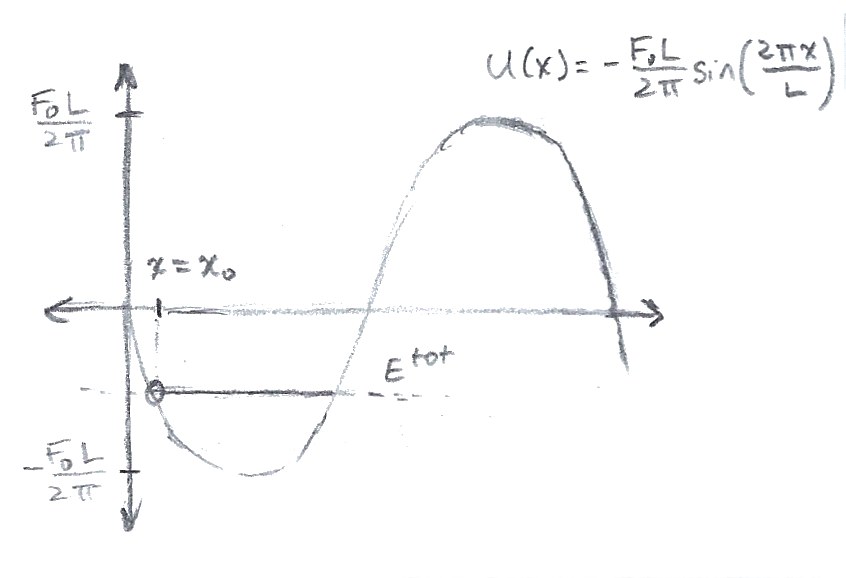
\includegraphics[width=0.5\textwidth]{images/mechintro/cons-energy-1.png}\\
\end{center}
Since there are no external forces on the system and the force is conservative, the energy in the system is conserved. On the graph, we can draw a horizontal line to show how much energy is in the system, as shown. Note that the particle can't reach any position that must cross above the line since otherwise, the system would have more energy than is actually in the system. Therefore, the motion of the particle is restricted to the interval that is bounded by the horizontal line and the potential energy curve. \\
Since potential energy can only be converted to kinetic energy (and vice versa), the particle has its maximum amount of kinetic energy when it has the least amount of potential energy. We can use calculus (or just know how sine functions work, to be honest) to conclude that minimum occurs at $x = \frac{L}{4}$. The potential energy at this point is then:
\[
	U\left(\frac{L}{4}\right) = - \frac{F_0L}{2\pi} \sin \left(\frac{2\pi L}{4L} \right) = - \frac{F_0L}{2\pi}
\]
The change in the potential energy is then:
\[
	\Delta U = U\left(\frac{L}{4}\right) - U(x_0)= \frac{F_0L}{2\pi} \sin \left(\frac{2\pi x_0}{L} \right) - \frac{F_0L}{2\pi}
\]
By conservation of energy, we have $- \Delta U = \Delta K$, so the change in kinetic energy $\Delta K$ is:
\[
	\Delta K = \frac{F_0L}{2\pi}\left(1 - \sin \left(\frac{2\pi x_0}{L} \right)\right)= \frac{1}{2}mv_{max}^2
\]
From this, we get the (pretty messy) expression for the maximum velocity of the particle:
\[
	v_{max} = \sqrt{\frac{F_0L}{\pi m}\left(1 - \sin \left(\frac{2\pi x_0}{L} \right)\right)}
\]
If we launch the particle at some velocity $v_0$, the total energy is higher, because the particle has its own kinetic energy to be accounted for. Let's find the minimum value of $v_0$ for the particle to never return. 
\begin{center}
	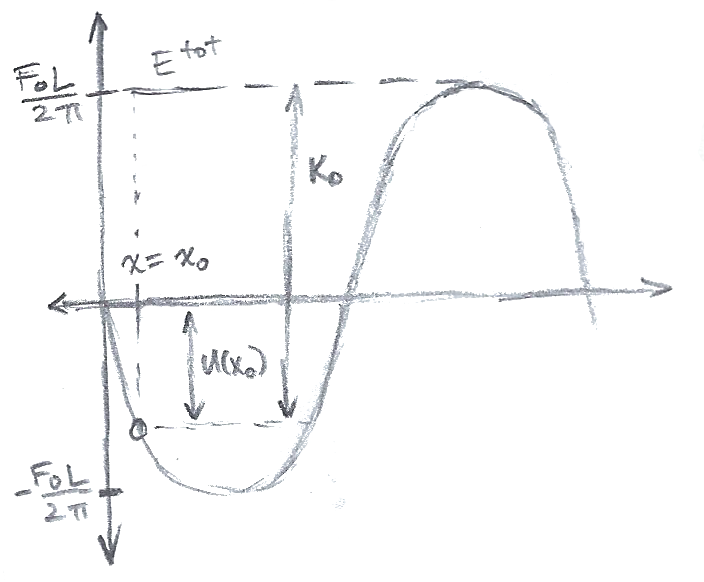
\includegraphics[width=0.4\textwidth]{images/mechintro/cons-energy-2.png}\\
\end{center}
If enough kinetic energy is given to the particle so that it escapes and never comes back to the starting point, the total energy should then be greater than or equal to the maximum value of the potential energy. This means:
\[
	\frac{1}{2}mv_0^2 - \frac{F_0L}{2\pi} \sin \left(\frac{2\pi x_0}{L} \right) = \frac{F_0L}{2\pi}
\]
We can solve and obtain the following expression for $v_0$:
\[
	v_0 = \sqrt{\frac{F_0L}{\pi m} \left(1 + \sin \left(\frac{2\pi x_0}{L} \right) \right)}
\]
The same principles of conservation of energy can be applied to general mechanical systems of a wide variety, as will be seen in the problems.  
\subsubsection{Summary and Problems}
The conservation of energy is a useful principle that can be applied widely to many problems where other dynamical information may not be available. In particular, it tends to provide a helpful link between velocity and position that is not readily attainable from momentum, dynamics, or kinematics. These problems may integrate concepts from all the other units as well - including collisions, which can be classified as elastic, completely inelastic, or partially inelastic. Elastic collisions conserve kinetic energy of the objects before and after the collision, completely inelastic collisions occur when the objects have the same velocity, and partially inelastic collisions satisfy neither of these conditions. Most problems that we will see will either concern a completely inelastic or elastic collision. As a final general rule of thum, remember that if energy is not conserved during a process, be sure to note where that energy goes, whether if it's lost to nonconservative forces such as friction or in a collision. \\

\noindent \textbf{Problems:}\\
1. (2 $\bigstar$) A box slides from rest down a frictionless ramp inclined at an angle $\theta$ with respect to the horizontal and is stopped at the bottom of the ramp by a spring with a spring constant of $k$. If the box has a mass of $m$ and slides a distance $d$ from the point of release to the point where it comes to rest against the spring, show the compression $x$ of the spring when the box comes to rest is $x = \sqrt{\frac{2mgd\sin\theta}{k}}$.\\
2. (3 $\bigstar$) A child of mass $m$ on a playground swing moves with a speed of $v_0$ when the swing of length $L$ is at its lowest point. Show that the angle $\theta$ that the swing makes with the vertical when the child is at the highest point is equal to $\theta = \arccos\left(1- \frac{v_0^2}{2gL}\right)$.\\
3. (3 $\bigstar$) A pendulum consists of a small bob of mass m attached to a string of length $L$. The bob is held to the side with the string horizontal. Then the bob is released from rest. At the lowest point of the swing, the string catches on a thin peg a distance $R$ above the lowest point. Show that $R$ must be smaller than $2L/5$ if the string is to remain taut as the bob swings around the peg in a full circle. \\
4. (2 $\bigstar$)  A small object of mass $m$ moves in a horizontal circle of radius $r$ on a rough table. It is attached to a horizontal string fixed at the center of the circle. The speed of the object is initially $v_0$. After completing one full trip around the circle, the speed of the object is $0.5v_0$. a) Show that the energy dissipated by friction during that one revolution is $\frac{3}{8}mv_0^2$. b) Show that the coefficient of kinetic friction is $\frac{3v_0^2}{16\pi gr}$. c) Show that the object will make a further $\frac{1}{3}$ of a revolution before coming to rest.\\
5. (3 $\bigstar$, $\spadesuit$) The potential energy of a diatomic molecule is given by the following expression with $r$ being the separation of the two atoms of the molecule and $A$ and $B$ being positive constants: $$U = A/r^{12} - B/r^6$$ This potential energy is associated with the force that binds the two atoms together. Show that the equilibrium distance $r$ where no net force acts on either molecule is $1.12(A/B)^{1/6}$.\\
6. (4 $\bigstar$) A pendulum consists of a compact 0.60 kg bob attached to a string of length 1.00 m. A block of mass $m$ rests on a horizontal frictionless surface. The pendulum is released from rest at an angle of 53$^\circ$ with the vertical. The bob collides elastically with the block at the lowest point in its arc. Following the collision, the maximum angle of the pendulum with the vertical is 5.73$^\circ$. Show that the mass $m$ can be equal to both 0.751 kg and 0.479 kg. \\
7. (3 $\bigstar$) A neutron of mass $m$ makes an elastic head-on collision with a stationary nucleus of mass $M$. a) Show that the kinetic energy of the nucleus after the collision is given by $K_{nucleus} = \frac{4Mm}{(m+M)^2}K_n$ where $K_n$ is the initial kinetic energy of the neutron. b) Show that the fractional change in the kinetic energy of the neutron is given by $\frac{\Delta K_n}{K_n} = -\frac{4(m/M)}{1+(m/M)^2}$.
\pagebreak

\subsection{Universal Gravitation}
The last section on mechanics will deal with gravity, starting with Newton's law of Universal Gravitation and looking at why this is consistent with Kepler's Laws of Planetary Motion.
\subsubsection{Newton's Law of Universal Gravitation}
From empirical observations, Newton posited the inverse-square law for gravity, where he claimed the force of gravity between two objects varied as the reciprocal of the square of the distance between the two.\\
\begin{center}
    \begin{asy}
        import geometry;
        size(8cm);
        
        draw(unitcircle);
        draw(shift(15, 0) * unitcircle);
        
        draw((0, -1.5)--(15, -1.5), linetype("8 8"), Arrows);
        draw((1,0)--(3,0), Arrow);
        draw((14,0)--(12,0), Arrow);
        
        label("$m_1$", (0, 1), N);
        label("$m_2$", (15, 1), N);
        label("$r_{12}$", (0, -1.5)--(15, -1.5), S);
        label("$\vec F_{12}$", (1,0)--(3,0), N);
        label("$\vec F_{21}$", (14,0)--(12,0), N);
    \end{asy}
\end{center}
Symbolically, if $m_1$ and $m_2$ are the masses of the two objects, $r_{12}$ is the distance between the two, and $\hat r_{12}$ is the unit vector in the direction from mass 1 to mass 2, then the gravitational force $\vec F_{21}$ on mass 2 due to mass 1 is:
\[
	\vec F = - \frac{Gm_1m_2}{r_{12}^2} \hat r_{12}
\]
The capital $G$ is not the acceleration due to gravity but is the universal gravitational constant that has the weird value of 6.674 $\cdot$ 10$^{-11}$ N$\cdot$m$^2$/kg$^2$. Notice that this formula also holds if you swap masses 1 and 2 - if we define $\hat r_{21}$ as the unit vector from mass 2 to mass 1 instead, so that $\hat r_{21} = - \hat r_{12}$, this still holds. As expected, the negative sign in front of the fraction is to ensure that this is an attractive force, since from real life we can clearly see that gravity pulls things together. 
\subsubsection{Gravitational Fields and Potential Energy}
Moving forward, we're going to work with different kinds of fields. Before moving on, I want to be clear as to what a field is - it's the assignment of some value to every point in space. Mostly, we're going to look at vector fields and scalar fields - fields where a vector/scalar are assigned to every point. The first ones we'll encounter in physics are the gravitational field and the gravitational potential. \\
Consider placing a very small test point particle $m_0$ amongst a collection of masses. These masses exert a gravitational force $\vec F_{net}$ on the particle:
\[
	\vec F_{net} = \sum_i \vec F_i = \sum_i -\frac{Gm_0m_i}{r_i^2}\hat r_i
\]
(For clarity - I'm using $m_i$ as the mass of the $i$th particle, $r_i$ for the distance between $m_0$ and $m_i$, and $\hat r_i$ as the unit vector in the direction from $m_0$ to $m_i$.)\\
Now, define the gravitational field at the position of the test mass $m_0$ as the net gravitational force divided by the mass of the small test particle:
\[
	\vec g = \frac{\vec F_{net}}{m_0} = \sum_i -\frac{Gm_i}{r_i^2}\hat r_i
\]
Notice for a single point mass, then, we have the gravitational field $\vec g = -\frac{Gm_i}{r^2}\hat r$ where $r$ is the distance from the point mass and $\hat r$ is just radially outward from the mass. However, more likely than not we are going to encounter continuous distributions of mass, which will require integration and superposing infinitely many small gravitational fields to create the total field. Here, we're going to derive the gravitational field due to a thin ring of mass and for a spherical shell. \\
\begin{center}
    \begin{asy}
        import three;
        size(6cm);
        triple eye = (7, 8, 5);
        currentprojection = perspective(eye);
        triple center = (0, 0, 0);
        real R = 1, y = 2;
        draw(circle(center, R, Z));
        dot((0, 0, y));
        real dqAngle = -20, dqDelta = 6;
        draw(arc(center, R,
                90, dqAngle - dqDelta,
                90, dqAngle + dqDelta), linewidth(2));
        draw(dir(90, dqAngle) -- (0, 0, y), linetype("6 6"));
        triple radiusPt = R * dir(90, 170);
        draw((0, 0, 0)--radiusPt, gray(0.2));
        draw((0, 0, 0)--(0, 0, y), gray(0.2));
        
        label("$M$", (0, R, 0), dir(-90));
        label("$m_0$", (0, 0, y), dir(130));
        label("$dM$", dir(90, dqAngle), dir(200));
        label("$R$", radiusPt/2, dir(-40));
        label("$y$", (0, 0, y/2), dir(0));
    \end{asy}
\end{center}
First, let's consider a uniform ring of mass $M$ and radius $R$, and for simplicity let's use a test mass $m_0$ on the axis of symmetry of the ring, at a distance of $y$ above the center. This ring has a linear mass density $\lambda = \frac{M}{2\pi R}$. We can consider dividing the ring into infinitely many tiny arcs, with length $ds = R \, d\theta$. The mass of this piece can then be shown to be $dm = \lambda R \, d\theta$. \\
From this, we conclude the magnitude of the force on the test mass from this small arc, $dF$, is
\[
    dF = \frac{Gm_0 \,dm}{R^2 + y^2}
\]
Note that the radial components of the force will cancel each other out by symmetry, so it suffices to consider the components of the force in the $y$-direction, $dF_y$:
\[
    dF_y = -\frac{Gm_0 \, dm}{R^2 + y^2} \cdot \frac{y}{\sqrt{R^2+y^2}} = \frac{Gm_0 \, dm \, y}{(R^2 + y^2)^{3/2}}.
\]
The negative sign is present since gravity is an attractive force. We can now integrate over all the small bits of mass: 
\begin{align*}
    F &= \int_0^{2\pi} dF_y \\
    &= \int_0^{2\pi} -\frac{Gm_0 \, dm \, y}{(R^2 + y^2)^{3/2}} \\
    &= \int_0^{2\pi} -\frac{Gm_0y \lambda R \, d \theta}{(R^2 + y^2)^{3/2}}\\
    &= -\frac{Gm_0My}{(R^2 + y^2)^{3/2}}.
\end{align*}
The force is directed in the negative $y$-direction, and thus the force is
\[
    \vec F = -\frac{Gm_0My}{(R^2 + y^2)^{3/2}}\hat y
\]
To find the gravitational field along the axis at any distance from the center $y$, we simply use our definition to find:
\[
    \vec g = \frac{GMy}{(R^2 + y^2)^{3/2}}\hat y.
\]
\begin{center}
    \begin{asy}
        import solids;
        import three;
        size(8cm);
        
        currentprojection=orthographic(0.7, -4, 1);
        currentlight=nolight;
        triple center = (0,0,0);
        triple ringctr = (0.5, 0, 0);
        real R=1, RS=0.7, inc=100, lat=45, lon=45, tlat=50, tlon=100;
        dot(center);
        real r = 2;
        dot(ringctr);
        revolution Earth=sphere(center, R);  
        
        draw(surface(Earth), surfacepen=white+opacity(.1), meshpen=0.7*black);
        draw(arc(ringctr, sqrt(3)/2, 0, 90, 180, 270), linewidth(2));
        draw(arc(ringctr, sqrt(3)/2, 180, 270, 0, 90), linewidth(2)+linetype("4 4"));
        dot((r, 0, 0));

        draw((0,0,0)--(r, 0, 0));
        draw(center--(0.5, 0, sqrt(3)/2));
        label("$R$", (0.25, 0, sqrt(3)/4), dir(120));
        label("$dM$", (0.5, 0, sqrt(3)/2), dir(40)*1.5);
        label("$\theta$", center, dir(30)*2);
        label("$r$", (r*0.75, 0, 0), dir(90));
        label("$m_0$", (r, 0, 0), dir(50));
    \end{asy}
\end{center}
From here, we can proceed to find the gravitational field of a uniform thin spherical shell of mass $M$ and radius $R$, making the surface density $\sigma = \frac{M}{4\pi R^2}$. Consider a test mass $m_0$, a distance $r$ away from the center of the sphere. We can split the sphere into many rings and use a scanning variable $\theta$ that represents the angle between the line joining the center to the edge of the ring and the horizontal. The surface area of each ring $dA = 2\pi R^2 \sin \theta \, d\theta$ (as seen before in the moment of inertia calculation), so then mass of each ring, $dm$, can be seen to be $dm = 2\pi \sigma R^2 \sin \theta \, d\theta$. We can then plug straight back into the formula for a ring to get: 
\[
    dF = \frac{Gm_0(r-R\cos \theta)\, dm}{((R\sin \theta)^2 + (r-R\cos \theta)^2)^{3/2}} = \frac{2Gm_0R^2 \pi \sigma (r-R\cos \theta) \sin \theta \, d\theta}{((R\sin \theta)^2 + (r-R\cos \theta)^2)^{3/2}}
\]
We integrate with respect to $\theta$ from $0$ to $\pi$, and simplify as much as possible: 
\begin{align*}
    F &= \int_0^\pi \frac{2Gm_0R^2 \pi \sigma (r-R\cos \theta) \sin \theta \, d\theta}{((R\sin \theta)^2 + (r-R\cos \theta)^2)^{3/2}}\\
    &= Gm_0\pi\sigma \int_0^\pi \frac{2R^2 (r-R\cos \theta) \sin \theta \, d\theta}{(R^2 + r^2 - 2rR\cos \theta)^{3/2}}
\end{align*}
Let $u = R^2 + r^2 - 2rR\cos \theta$, and $du = 2rR \sin \theta \, d\theta$, which changes the bounds to $(r-R)^2$ to $(r+R)^2$. From this, we also get that $\cos \theta = \frac{R^2+r^2-u}{2Rr}$ and gives
\begin{align*}
    F &= Gm_0\pi\sigma \int_{(r-R)^2}^{(r+R)^2} \frac{R}{r} \left(r-\frac{R^2+r^2-u}{2r}\right) u^{-\frac{3}{2}}\, du \\
    &= \frac{Gm_0\pi\sigma R}{2r^2} \int_{(r-R)^2}^{(r+R)^2} (r^2-R^2+u) u^{-\frac{3}{2}}\, du \\
    &= \frac{Gm_0\pi\sigma R}{2r^2} \int_{(r-R)^2}^{(r+R)^2} (r^2-R^2)u^{-\frac{3}{2}} + u^{-\frac{1}{2}}\, du \\
    &= \frac{Gm_0\pi\sigma R}{2r^2} (-2(r^2-R^2)u^{-\frac{1}{2}} + 2u^{\frac{1}{2}}) \Big|_{(r-R)^2}^{(r+R)^2} \\
    &= \frac{Gm_0\pi\sigma R}{r^2} ((R^2-r^2)u^{-\frac{1}{2}} + u^{\frac{1}{2}}) \Big|_{(r-R)^2}^{(r+R)^2}\\
\end{align*}
\textbf{Case 1: Outside the Shell} \newline
Assume now that $r > R$, so $r - R> 0$. Evaluating, we have
\begin{align*}
    F &= \frac{Gm_0\pi\sigma R}{r^2} \left(\frac{R^2-r^2}{r+R} + R+r - \frac{R^2-r^2}{r-R} - (r - R)\right) \\
    &= \frac{Gm_0\pi\sigma R}{r^2} (R-r + R+r + R+ r + R -r)\\
    &= \frac{Gm_0\pi\sigma 4R^2}{r^2} \\
    &= \frac{Gm_0Q}{r^2} 
\end{align*}
From this, we see that 
\[
    \vec g = \frac{GM}{r^2}\hat r
\]
where $\hat r$ is the unit vector radially outward from the center of the sphere to the point charge. \\ 
\textbf{Case 2: Inside the Shell} \\
Assume now that $r < R$, so $R - r> 0$. Evaluating, we have
\begin{align*}
    F &= \frac{Gm_0\pi\sigma R}{r^2} \left(\frac{R^2-r^2}{r+R} + R+r - \frac{R^2-r^2}{R-r} - (R-r)\right) \\
    &= \frac{Gm_0\pi\sigma R}{r^2} (R-r + R+r - R - r -R + r)\\
    &= 0
\end{align*}
and clearly $\vec g = 0$. Notice that outside the shell, the field is exactly the same as if the shell was essentially a point mass, and on the inside, it's zero. This is a result known as the Shell Theorem. \\
Another field that we will investigate is a scalar field, the potential energy field. First, let's look at the gravitational potential energy of a mass $m_0$ brought from arbitrarily far away (so, basically infinity) to a distance $r$ away from a mass $M$. Assuming the potential energy at infinity is zero, the potential energy function $U(r)$ is then:
\[
	U = - \int_r^{\infty} F \, dr = - \int_r^{\infty} -\frac{Gm_0M}{r^2} \, dr = -\frac{Gm_0M}{r}
\]
This also follows the principles of superposition that is true for gravitational fields, but direction need not be taken into account because energy is a scalar. For reference, here are the potential energies of a test particle $m_0$ near the ring and shell:
\[
	U = -\frac{GMm_0}{\sqrt{R^2 + y^2}} \quad U = -\frac{Gm_0M}{r}
\]
\subsubsection{Kepler's Laws of Planetary Motion}
Before Newton, Kepler proposed three laws of planetary motion from empirical data of the positions of astronomical bodies as they orbited the sun. These are the laws Kepler proposed: \\
1. All planets orbit around a sun in elliptical orbits with the sun at one focus of the ellipse.\\
2. Planets sweep out equal-sized areas in equal time intervals. \\
3. The square of the period of a planet's orbit is proportional to the cube of the semi-major axis of the planet's orbit: more specifically, 
\[
	T^2 = \frac{4\pi^2}{GM} a^3
\]
where $M$ is the mass of the sun. \\
% \section*{Appendix A: Proof of Kepler's Laws}
% \addcontentsline{toc}{section}{Appendix A: Proof of Kepler's Laws}
% As a reminder, here is a restatement of Kepler's Laws:\\
% 1. All planets orbit around a sun in elliptical orbits with the sun at one focus of the ellipse.\\
% 2. Planets sweep out equal-sized areas in equal time intervals. \\
% 3. The square of the period of a planet's orbit around a mass $M$ is proportional to the cube of the semi-major axis of the planet's orbit: more specifically, 
% \[
% 	T^2 = \frac{4\pi^2}{GM} a^3
% \]
The first and third statements follow from Newton's Law of Universal Gravitation, but the second is essentially a disguised conservation of angular momentum (see the problems from Rotation!). We're going to prove these two using Newton's Law of Universal Gravitation and Newton's Second Law of Motion. \\
\begin{center}
	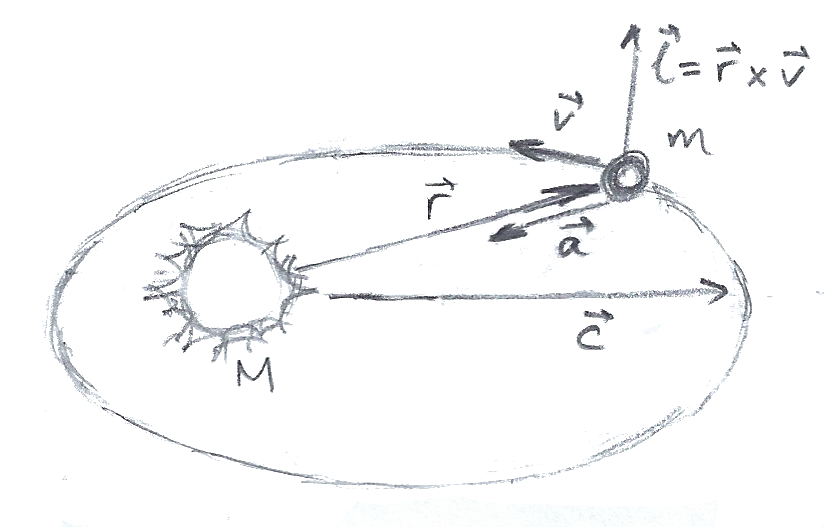
\includegraphics[width=0.5\textwidth]{images/mechintro/kepler-1.png}\\
\end{center}
If a satellite of mass $m$ is orbiting around a mass $M$, the force $\vec F = - \frac{GmM}{r^2} \hat r$ where $\hat r$ and $r$ are varying with time. Because of this, notice that $\vec a =  - \frac{GM}{r^2} \hat r$ from Newton's Second Law. The position $\vec r$ and $\vec a$ are then always in the same direction. \\
Assuming no other forces act on the system, the orbital angular momentum $\vec L = \vec r \times m \vec v$ is constant. We're more interested in the fact that the cross product $\vec r \times \vec v$ is also a constant, so we're going to denote this by $\vec l$. But what exactly is $\vec l$? We can do this explicitly:
\begin{align*}
	\vec l &= \vec r \times \vec v \\
	&= \vec r \times \dv{\vec r}{t}\\
	&= r \hat r \times \dv{}{t}(r \hat r)\\
	&= r \hat r \times (r' \hat r + r \hat r')\\
	&= r^2(\hat r \times \hat r')\\
\end{align*}
We're going to do something a little contrived: what happens when we take $\vec a \times \vec l$? We can use the triple vector product identity to help us out, and the fact that we've decomposed everything into unit vectors with magnitude 1:
\begin{align*}
	\vec a \times \vec l &=  - \frac{GM}{r^2} \hat r \times r^2 (\hat r \times \hat r')\\
	&= -GM [ \hat r (\hat r \cdot \hat r') - \hat r' (\hat r \cdot \hat r) ]\\
	&= GM \hat r'
\end{align*}
The first dot product in parentheses is zero - the derivative of a unit vector is always perpendicular to the original. If you're not convinced, look at $\hat r$ and $\hat \theta$ when we derived circular motion - $\hat \theta$ is proportional to the derivative of $\hat r$, and $\hat \theta \cdot \hat r = 0$. \\
Since we know how $\vec a \times \vec l$, we can find $\vec v \times \vec l$. Considering that 
\[
	\dv{}{t} (\vec v \times \vec l) = \dv {\vec v}{t} \times l + \vec v \times \dv{\vec l}{t} = \vec a \times \vec l + \vec v \times \vec 0 = \vec a \times \vec l
\]
we can integrate to find $\vec v \times \vec l = GM \hat r + \vec c$ for some constant vector $\vec c$. \\
We have one more contrived step to take: consider $\vec r \cdot (\vec v \times \vec l)$. We can expand it as follows:
\begin{align*}
	\vec r \cdot (\vec v \times \vec l) &= \vec r \cdot (GM \hat r + \vec c) \\
	&= GM (\vec r \cdot \hat r) + \vec r \cdot \hat c\\
	&= GMr + rc \cos \theta
\end{align*}
where $\theta$ is the angle between $\vec r$ and $\vec c$. On the other hand, since this is a scalar triple product, $\vec r \cdot (\vec v \times \vec l) = \vec l \cdot (\vec r \times \vec v) = \vec l \cdot \vec l = l^2$. Therefore, 
\[
	l^2 = GMr + rc \cos \theta
\]
\[
	r = \frac{l^2}{GM + c \cos \theta} = \frac{\frac{l^2}{GM}}{1 + \frac{c}{GM} \cos \theta}
\]
That is the polar equation for an ellipse, centered at one of its foci (if you might recall from the conics unit), and this gives Kepler's First Law.\\
\begin{center}
	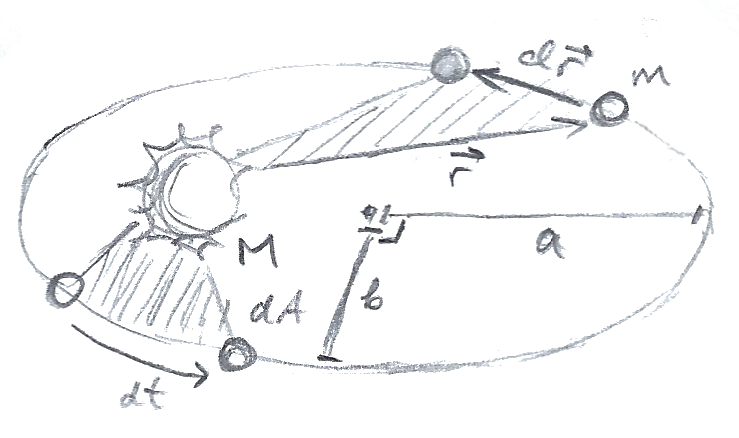
\includegraphics[width=0.5\textwidth]{images/mechintro/kepler-2.png}\\
\end{center}
For Kepler's Second Law, we reuse the fact that $\vec l = \vec r \times \vec v$ is a constant. Consider a small triangular area $dA$ swept out in a time $dt$ by a satellite. This area $dA = \frac{1}{2}| \vec r \times d\vec r |$, where $d\vec r$ is the displacement of the satellite. Dividing by $dt$ gives $\dv{A}{t} = \frac{1}{2} \left| \vec r \times \dv{\vec r}{t} \right| = \frac{1}{2} \left| \vec r \times \vec v \right| = \frac{1}{2} l$. Since $\vec l$ is constant, we have that the area swept out per unit time is constant, so the area swept out by a satellite in a given time interval is also a constant. \\
Using this, we can prove Kepler's Third Law. The rate at which area is swept out is $\dv{A}{t} = \frac{1}{2} l$ by Kepler's Second Law, but since this is constant it's also equal to the total area of the elliptical orbit over the period of the motion. Letting $a$ and $b$ be the lengths of the semi-major and semi-minor axes, we have 
\[
	\dv{A}{t} = \frac{\pi a b}{T} = \frac{1}{2}l
\]
From this, we see that 
\[
	T = \frac{2\pi a b}{l} \rightarrow T^2 = \frac{4\pi^2 a^2 b^2}{l^2}
\]
I'm going to gloss over this part a little bit - but recall that an ellipse in polar coordinates is defined by its eccentricity $e$ and the distance from the focus to the directrix $d$. The computation is extremely messy, but it can be shown (with great effort) that the numerator of the polar equation $ed = \frac{b^2}{a}$. In this case, then, $\frac{l^2}{GM} = \frac{b^2}{a}$, which is equivalent to $\frac{b^2}{l^2} = \frac{a}{GM}$. We can plug this back in to get
\[
	T^2 = \frac{4\pi^2}{GM}a^3
\]
This shows Kepler's Third Law. Usually, however, we won't work with actual elliptical orbits - most of the time we will just deal with simplified circular orbits, where the semi-major axis is just the radius of the circle. 
These equations hold true in general for satellites orbiting around large masses, if the satellite's mass is negligible - otherwise, one must consider orbit around the center of mass and use the total mass for Kepler's Third Law. We will see why this is as a problem at the end of the chapter.
\subsubsection{Summary and Problems} 
Using Newton's Law of Gravitation and our knowledge of mechanics up to this point, we derived Kepler's Laws and we can now apply them in these problems. As a result of Newton's Law of Gravitation, we were also able to derive a gravitational field which we will calculate for a few setups. We can also look at the potential energy of gravitational fields, which we will also explore a little. \\

\noindent\textbf{Problems:}\\
1. (1 $\bigstar$) Given that the mean period of the Moon's orbit is 27.3 days, the mean orbital radius of the Moon around the Earth is 385,000 km, and the value of $G$, approximate the mass of the Earth to be about 6.07$\cdot$10$^{24}$ kg. \\
2. (2 $\bigstar$, $\spadesuit$) Two particles, each of mass $M$, are fixed in position on the $y$-axis at $y = +a$ and $y = -a$. Show that on the $x-$axis, the maximum value of $g$ for the gravitational field occurs at points $x = \pm a/\sqrt{2}$. \\
3. (3 $\bigstar$) An object is projected vertically from the surface of Earth at less than the escape speed. Show that the maximum height $H$ reached by the object is $H = \frac{R_EH'}{R_E - H'}$, where $H'$ is the height that it would reach if the gravitational field were constant, and $R_E$ is the radius of the Earth. Notice that for large values of the launch velocity for a projectile, this model is more precise if significant fluctuations in the gravitational field are observed over the course of the object's flight.\\
4. (4 $\bigstar$, $\spadesuit$) A uniform thin rod of mass $M$ and length $L$ lies on the $+x$-axis with one end at the origin. Consider an element of the rod of length $dx$, and mass $dm$, at point $x$, where $0<x<L$. a) Show that this element produces a gravitational field $dg_{x}$ at a point $x_0$ on the $x-$axis in the region $x_0 > L$ is given by $dg_{x} = -\frac{GM}{L(x_0-x)^2}$. b) Show that the total gravitational field at the point $x_0$ due to the rod is $g = \frac{GM}{x_0(x_0-L)}$. c) Show that for $x_0 >> L$, the field of the rod approximates the field of a point particle of mass $M$ at $x = 0$. d) Using a similar method, compute the gravitational potential energy of a mass $m_0$ at a position $x_0$ to be $U = -\frac{GMm_0}{L} \ln\left(\frac{x_0+L/2}{x_0-L/2}\right)$.\\
5. (3 $\bigstar$) In a binary star system, two stars follow circular orbits about their common center of mass. If the stars have masses $m_1$ and $m_2$ and are separated by a distance $r$, show that the period of rotation is related to $r$ by $T^2 = \frac{4\pi^2}{G(m_1+m_2)}r^3$. \\
6. (2 $\bigstar$) Four identical planets are arranged in a square of side length $a$. If the mass of each planet is $M$, show that the speed of each planet is $v = \sqrt{\frac{GM}{a}\left(\frac{\sqrt{2}}{4} + 1 \right)}$ if they are to orbit their common center under the influence of their mutual attraction.\\
7. (3 $\bigstar$) Two particles of masses $m_1$ and $m_2$ are released from rest at a large separation distance. Show that their speeds $v_1$ and $v_2$ when their separation distance is $r$ are $v_1 = \sqrt{\frac{2Gm_2^2}{r(m_1+m_2)}}$ and $v_2 = \sqrt{\frac{2Gm_1^2}{r(m_1+m_2)}}$.
\pagebreak

\section*{Mechanics Highlights}
\addcontentsline{toc}{section}{\protect\numberline{}Mechanics Highlights}
Some of my personal favorite mechanics problems. These are hard problems, but I strongly encourage you to give most of these a try (except problem 1), because they're good problems. If you feel like you've attempted a problem several times and come up with an incorrect answer, I'd be happy to discuss these with you and go over them. \\
\textbf{Problems:}\\
1. (?? $\bigstar$) Find as many mistakes/inaccuracies as you can find in the Mechanics section. \\
2. (4 $\bigstar$) A solid bowling ball of mass $M$ and radius $R$ has an initial clockwise angular velocity $\omega_0$ down the lane and an initial speed of the the center of mass of the ball $s = \frac{R\omega_0}{3}$ just after its release. The coefficient of kinetic friction is $\mu_k$. Show that the final angular momentum of the ball about its initial point of contact with the floor is $\frac{11}{15}MR^2 \omega_0$.\\
3. (3 $\bigstar$) Consider a solid cylinder that has mass $M$ and radius $R$ to which a second solid cylinder that has mass $m$ and radius $r$ is attached. These cylinders share an axis of symmetry. A string is wound about the smaller cylinder. The larger cylinder rests on a horizontal surface. The coefficient of static friction between the larger cylinder and the surface is $\mu_k$. If a light tension is applied to the string in the vertical direction, the cylinder will roll to the left; if the tension is applied with the string horizontally to the right, the cylinder rolls to the right. Show that the angle between the string and the horizontal that will allow the cylinder to remain stationary when a
light tension is applied to the string is $\theta = \arccos \frac{r}{R}$. \\
4. (3 $\bigstar$) A boy is initially seated on the top of a hemispherical ice mound of radius $R$. He begins to slide down the ice, with a negligible initial speed. Approximate the ice as being frictionless. Show that the height where the boy loses contact with the ice is $\frac{2}{3}R$. \\
5. (4 $\bigstar$, $\spadesuit$) A rod of mass $M$ and length $L$ acts as a solid pendulum. Its pivot point is set a distance $d$ from its center of mass (in the center of the rod). Show that if the rod is set swinging (at small angles) and exhibits simple harmonic motion, the period of the motion can be maximized by setting $d = \frac{L}{2\sqrt{3}}$. Hint: Use blasphemy - $\sin \theta = \theta$ for small values of theta :P. \\
6. (5 $\bigstar$) A long rod of mass $M$ and length $L$ is at rest on a frictionless horizontal surface. A small blob of mass $M$ moving at a speed $s$ strikes the rod at one of its ends, and sticks to the rod. Show that the ratio of the total kinetic energy in the system before the collision to the total kinetic energy after the collision is $\frac{4}{5}$. \\
7. (4 $\bigstar$) A uniform rod with mass $M$ and length $L$ turns without friction on a fixed pivot at the end of the rod. The rod is released from rest from a horizontal position. The rod swings down, collides with a small dense block, also with mass $M$, and the block sticks to the end of the rod. Show that the maximum angular displacement of the rod from the vertical after the collision is $\theta = \arccos\left(\frac{11}{12}\right)$.\\
8. (5 $\bigstar$, $\spadesuit$) Two small blocks with masses $M$ and $2M$ are attached to a spring with negligible mass, spring constant $k$, and natural length $L$. The blocks and spring rest on a frictionless horizontal surface with the lighter block in contact with a wall located at $x=0$. The system is released from rest at time $t=0$ with the spring compressed to a length $\frac{L}{2}$. Show that the maximum length of the spring after the lighter block leaves the wall is $\left(1 + \frac{1}{2\sqrt{3}}\right) L$ and the location of the center of mass of the two-block system when this occurs is $\frac{\pi\sqrt{3}+2}{3}L$.
\pagebreak
